% VLDB-Template enhances the ACM master template, acmart.cls v2.19 (2026/06/27):
% https://github.com/vldbproceedings/VLDB-Template

\documentclass[sigconf, nonacm]{acmart}

%%% do not modify the following VLDB block %%
%%% VLDB block start %%%
\usepackage{pvldb}% VLDB/PVLDB formatting overrides, see pvldb.sty for details.
                      % Do not remove -- required for consistent proceedings
                      % formatting across all VLDB submissions.
%%% VLDB block end %%%

\renewcommand\vldbdoi{XX.XX/XXX.XX}
\renewcommand\vldbpages{XXX-XXX}
\renewcommand\vldbavailabilityurl{https://github.com/ZardLi1115/PiT-Mem}

\usepackage{booktabs}
\usepackage{multirow}
\usepackage{graphicx}
\usepackage{subcaption}
\usepackage{algorithm}
\usepackage{algpseudocode}
\usepackage{amsmath}
\usepackage{amsthm}
\usepackage{balance}
\usepackage{xcolor}
\usepackage{xurl}

\newtheorem{theorem}{Theorem}
\newtheorem{lemma}{Lemma}
\newtheorem{definition}{Definition}
\newtheorem{proposition}{Proposition}

% Experimental metric & table macros auto-generated from archived benchmark CSVs
% Auto-generated by pit_mem.plotting.generate_latex_macros — DO NOT EDIT MANUALLY
\newcommand{\ColabGPUName}{NVIDIA A100-SXM4-80GB}
\newcommand{\ColabVRAMGB}{80.0}
\newcommand{\ColabCPUCores}{12}
\newcommand{\ColabRAMTotal}{167 GiB}
\newcommand{\MaxCorpusScale}{2{,}000{,}000}
\newcommand{\UniqueSeedPassages}{431{,}217}
\newcommand{\HFUniquePassages}{394{,}529}
\newcommand{\CorpusExpansionFactor}{4.6\times}
\newcommand{\CorpusNearCloneRate}{0.18\%}
\newcommand{\CorpusNNOneCosPfk}{0.73}
\newcommand{\IntraLineageSECCosPfk}{0.95}
\newcommand{\IntraLineageSECCosPninety}{0.97}
\newcommand{\IntraLineageEvolveCosPfk}{1.00}
\newcommand{\CoreIndexBytesPerRec}{1{,}032}
\newcommand{\CoreIndexRAMGiB}{1.92}
\newcommand{\MmapFPThirtyTwoGiB}{5.72}

% Exp 1 Workload 1A: Moderate Selectivity (~12%, 100% Dual-Budget Causal Graph)
\newcommand{\ModSelectivityPct}{12.0\%}
\newcommand{\ModGraphTriggerPct}{100\%}
\newcommand{\ModPiTFastQPS}{493}
\newcommand{\ModPiTFastPnnMs}{2.97}
\newcommand{\ModPiTFastRecall}{90.5\%}
\newcommand{\ModPiTMaxQPS}{283}
\newcommand{\ModPiTMaxQPSConc}{3{,}160}
\newcommand{\ModPiTMaxMeanMs}{3.53}
\newcommand{\ModPiTMaxPfkMs}{3.49}
\newcommand{\ModPiTMaxPnnMs}{4.92}
\newcommand{\ModPiTMaxRecall}{93.1\%}
\newcommand{\ModPiTPeakQPS}{157}
\newcommand{\ModPiTPeakPnnMs}{8.47}
\newcommand{\ModPiTPeakRecall}{95.2\%}
\newcommand{\ModGridScanQPS}{31}
\newcommand{\ModGridScanPnnMs}{32.66}
\newcommand{\ModSpeedupVsGridQPS}{9.0\times}
\newcommand{\ModSpeedupVsGridFastQPS}{15.7\times}
\newcommand{\ModSpeedupVsGridPeakQPS}{5.0\times}
\newcommand{\ModSpeedupVsGridPnn}{6.6\times}
\newcommand{\ModACORNQPS}{46}
\newcommand{\ModACORNPnnMs}{29.35}
\newcommand{\ModACORNRecall}{93.1\%}
\newcommand{\ModSpeedupVsACORNQPS}{6.1\times}
\newcommand{\ModSpeedupVsACORNPnn}{6.0\times}
\newcommand{\ModSeRFRecall}{87.0\%}
\newcommand{\ModDSGRecall}{87.0\%}
\newcommand{\ModPGMaxQPS}{132.8}
\newcommand{\ModPGMaxPnnMs}{10.96}
\newcommand{\ModPGMaxRecall}{94.4\%}
\newcommand{\ModSpeedupVsPGMaxQPS}{2.1\times}
\newcommand{\ModSpeedupVsPGMaxPnn}{2.2\times}

% Exp 1 Workload 1B: Sparse Historical Audit (~1.0%)
\newcommand{\PiTMaxQPS}{565}
\newcommand{\PiTMaxQPSConc}{2{,}935}
\newcommand{\SparseRouterGraphPct}{0\%}
\newcommand{\GridScanSparseMaxQPS}{536}
\newcommand{\GridScanSparseMaxPnnMs}{2.28}
\newcommand{\PiTMaxMeanMs}{1.77}
\newcommand{\PiTMaxPfkMs}{1.75}
\newcommand{\PiTMaxPnnMs}{2.15}
\newcommand{\PiTMaxRecall}{100.0\%}
\newcommand{\PiTBuildSec}{183.9}
\newcommand{\PiTMemMB}{7{,}827}
\newcommand{\PiTMemGiB}{7.64}
\newcommand{\PiTMemGB}{8.21}
\newcommand{\PiTMinScaleQPS}{10{,}135}
\newcommand{\PiTMinScalePnnMs}{0.12}
\newcommand{\PiTMidScaleQPS}{2{,}308}
\newcommand{\PiTMidScalePnnMs}{0.45}
\newcommand{\PiTMidBuildSec}{51.3}
\newcommand{\PGMaxScale}{2{,}000{,}000}
\newcommand{\PGMinQPS}{54.5}
\newcommand{\PGMinPnnMs}{32.54}
\newcommand{\PGQPS}{45.8}
\newcommand{\PGPnnMs}{33.94}
\newcommand{\PGMaxScaleQPS}{72.5}
\newcommand{\PGMaxScalePnnMs}{31.76}
\newcommand{\PGRecall}{94.0\%}
\newcommand{\PGMidBuildSec}{256.6}
\newcommand{\PGMaxBuildSec}{921.5}
\newcommand{\PGBuildSpeedup}{5.0\times}
\newcommand{\SpeedupPGMinQPS}{186\times}
\newcommand{\SpeedupPGMinPnn}{266\times}
\newcommand{\SpeedupVsPGQPS}{50.4\times}
\newcommand{\SpeedupVsPGPnn}{76.2\times}
\newcommand{\SpeedupPGMaxQPS}{7.8\times}
\newcommand{\SpeedupPGMaxPnn}{14.8\times}
\newcommand{\ACORNSparseQPS}{15.3}
\newcommand{\ACORNSparsePnnMs}{76.64}
\newcommand{\ACORNSparseRecall}{88.0\%}
\newcommand{\HNSWMaxQPS}{117}
\newcommand{\HNSWMaxPnnMs}{14.95}
\newcommand{\HNSWMaxRecall}{94.9\%}
\newcommand{\SeRFMaxRecall}{80.1\%}
\newcommand{\DSGMaxRecall}{78.5\%}
\newcommand{\SpeedupVsHNSWPnn}{6.9\times}

% Exp 2 Selectivity Sweep
\newcommand{\ExpTwoScale}{1{,}000{,}000}
\newcommand{\NarrowPitQPS}{8{,}974}
\newcommand{\NarrowPitPnnMs}{0.17}
\newcommand{\NarrowPitRecall}{100.0\%}
\newcommand{\NarrowHNSWRecall}{54.0\%}
\newcommand{\NarrowHNSWPnnMs}{10.45}
\newcommand{\NarrowACORNRecall}{32.5\%}
\newcommand{\NarrowACORNPnnMs}{6.73}
\newcommand{\NarrowSeRFRecall}{38.1\%}
\newcommand{\BroadPitRecall}{89.8\%}
\newcommand{\BroadPitPnnMs}{3.38}
\newcommand{\BroadPitQPS}{422}
\newcommand{\BroadScanPnnMs}{51.05}
\newcommand{\BroadScanQPS}{20}
\newcommand{\BroadScanSpeedup}{15.1\times}

% Exp 3 Restatement & End-to-End Write+Read Token Cost
\newcommand{\RestateWriteOps}{1{,}012}
\newcommand{\RestateWritePfkUs}{904.5}
\newcommand{\RestateWritePnnUs}{1{,}580.1}
\newcommand{\RestateEagerOps}{1.6}
\newcommand{\RestateEagerOpsTwentyPct}{0.8}
\newcommand{\RestateStaticOps}{22.3}
\newcommand{\AvgTokenSavings}{75.7\%}
\newcommand{\UnpackOnlySavings}{1.6\%}
\newcommand{\LazyWriteTokensTenPct}{294{,}106}
\newcommand{\LazyReadExtraTokensTenPct}{188{,}486}
\newcommand{\UnpackReadExtraTokensTenPct}{2{,}427{,}980}
\newcommand{\EagerWriteTokensTenPct}{1{,}916{,}000}

% Exp 4 Leakage & Audit
\newcommand{\PiTLCR}{0.00\%}
\newcommand{\PiTAuditFOneA}{71.2\%}
\newcommand{\PiTAuditFOneB}{66.7\%}
\newcommand{\NoLazyStaleA}{80.0\%}
\newcommand{\NoLazyStaleB}{100.0\%}
\newcommand{\NoLazyFOneA}{11.9\%}
\newcommand{\NoLazyFOneB}{0.0\%}
\newcommand{\GraphitiLCR}{72.5\%}
\newcommand{\GraphitiLCRB}{50.0\%}
\newcommand{\GraphitiSharpeInfl}{+0.25}
\newcommand{\MemZeroLCR}{99.2\%}
\newcommand{\MemZeroFOneA}{62.9\%}
\newcommand{\MemZeroFOneB}{34.1\%}
\newcommand{\MemZeroSharpeInfl}{+4.35}
\newcommand{\NaiveRAGLCRA}{68.3\%}
\newcommand{\NaiveRAGLCRB}{71.7\%}

% Exp 5 RAP-Compact vs Parquet-Zstd, SQLite-BTree & Wild SEC EDGAR
\newcommand{\RAPCompRatio}{13.2\times}
\newcommand{\RAPMaxCompRatio}{15.7\times}
\newcommand{\RAPCovenantQA}{100.0\%}
\newcommand{\RAPQueryLatUs}{8.4}
\newcommand{\ParquetCompRatio}{8.6\times}
\newcommand{\ParquetQueryLatUs}{1{,}929}
\newcommand{\SQLiteCompRatio}{4.3\times}
\newcommand{\SQLiteQueryLatUs}{43.4}
\newcommand{\RAPSpeedupVsParquet}{230\times}
\newcommand{\RAPSpeedupVsSQLite}{5.2\times}
\newcommand{\WildSECAcc}{100.0\%}
\newcommand{\WildSECCompRatio}{18.5\times}
\newcommand{\WildSECQueryLatUs}{9.0}
\newcommand{\LLMSumCovenantQA}{1.5\%}
\newcommand{\MeanPoolCovenantQA}{18.0\%}

% Exp 3B: 3-Hop Clustered Restatement Burst (Static vs Adaptive k_fetch Doubling)
\newcommand{\BurstTwentyFourStaticRecall}{10.0\%}
\newcommand{\BurstTwentyFourAdaptRecall}{100.0\%}
\newcommand{\BurstThirtyTwoStaticRecall}{10.0\%}
\newcommand{\BurstThirtyTwoAdaptRecall}{100.0\%}
\newcommand{\BurstThirtyTwoAdaptRounds}{1.05}
\newcommand{\BurstThirtyTwoAdaptPnnMs}{1.20}

% Exp 5C: Unified Hot+Cold Tiered Search (query_tiered_pit)
\newcommand{\TieredHotOnlyQA}{42.0\%}
\newcommand{\TieredColdOnlyQA}{50.0\%}
\newcommand{\TieredUnifiedQA}{90.0\%}
\newcommand{\TieredUnifiedHitRate}{90.0\%}
\newcommand{\TieredUnifiedMeanUs}{17.0}
\newcommand{\TieredUnifiedPnnUs}{29.9}
\newcommand{\TieredUnifiedSTR}{0.0\%}

% Exp 6 Streaming Macro-Segments & NVMe Persistence
\newcommand{\StreamScale}{1{,}000{,}000}
\newcommand{\FrozenCellPileupPct}{95.1\%}
\newcommand{\FrozenQPS}{851}
\newcommand{\FrozenPnnMs}{1.23}
\newcommand{\StreamSegments}{4}
\newcommand{\StreamSealedMaxCellPct}{6.7\%}
\newcommand{\StreamCorpusMaxCellPct}{7.0\%}
\newcommand{\StreamMaxCellPct}{7.8\%}
\newcommand{\StreamQPS}{3{,}153}
\newcommand{\StreamPnnMs}{0.36}
\newcommand{\StreamSpeedupVsFrozen}{3.7\times}
\newcommand{\OracleQPS}{2{,}957}
\newcommand{\OraclePnnMs}{0.39}
\newcommand{\NVMeSnapGiB}{7.46}
\newcommand{\NVMeSaveSec}{26.2}
\newcommand{\NVMeSaveMiBs}{292}
\newcommand{\NVMeLoadWarmSec}{6.40}
\newcommand{\NVMeLoadWarmGiBs}{1.17}
\newcommand{\NVMeWALReplayMs}{68.8}

% Exp 6C: NVMe mmap Cold-FP32 Offload (1,032 B/rec Core Index RAM)
\newcommand{\OffloadWriteMBs}{256}
\newcommand{\OffloadAllRamModQPS}{277}
\newcommand{\OffloadAllRamModConcQPS}{1{,}839}
\newcommand{\OffloadAllRamSparseQPS}{599}
\newcommand{\OffloadAllRamSparseConcQPS}{3{,}184}
\newcommand{\OffloadWarmModQPS}{281}
\newcommand{\OffloadWarmModConcQPS}{1{,}882}
\newcommand{\OffloadWarmModPnnMs}{5.01}
\newcommand{\OffloadColdModQPS}{86}
\newcommand{\OffloadColdModQPSConc}{250}
\newcommand{\OffloadColdModPnnMs}{14.38}
\newcommand{\OffloadColdModRecall}{93.3\%}
\newcommand{\OffloadWarmSparseQPS}{628}
\newcommand{\OffloadWarmSparseConcQPS}{3{,}339}
\newcommand{\OffloadWarmSparsePnnMs}{1.88}
\newcommand{\OffloadColdSparseQPS}{281}
\newcommand{\OffloadColdSparseQPSConc}{944}
\newcommand{\OffloadColdSparsePnnMs}{4.94}
\newcommand{\OffloadColdSparseRecall}{100.0\%}

% Exp 6D: Multi-Threaded Concurrent Readers + Streaming Insert/Restate/Rollover
\newcommand{\ConcScale}{500{,}000}
\newcommand{\ConcTwelveROQPS}{2{,}547}
\newcommand{\ConcTwelveROPnnMs}{7.67}
\newcommand{\ConcTwelveMixedQPS}{1{,}613}
\newcommand{\ConcTwelveMixedPfkMs}{7.31}
\newcommand{\ConcTwelveMixedPnnMs}{13.04}
\newcommand{\ConcTwelveWriterOps}{134}
\newcommand{\ConcEightMixedQPS}{1{,}364}
\newcommand{\ConcEightMixedPnnMs}{10.00}
\newcommand{\ConcEightWriterOps}{170}
\newcommand{\ConcPerRunRollovers}{1}
\newcommand{\ConcTotalRollovers}{4}
\newcommand{\ConcTotalViolations}{0}

% Auto-generated LaTeX tables from experimental CSVs
\newcommand{\TableExpOne}{%
\begin{table*}[t]
\centering
\caption{Exp 1: Single-thread wall-clock QPS ($\text{QPS} = N_q / T_{\text{wall}}$), Mean/P50/P99 latency, Recall@10, causal-graph trigger share, build time, and memory footprint up to $N = \MaxCorpusScale$ under Workload 1A ($\sigma \approx 12\%$) and Workload 1B ($\sigma \approx 1.0\%$). For PiT-Mem, we report All-RAM total alongside the \CoreIndexBytesPerRec~B/rec core index array footprint (at 2M: $ef=192$ on W1A, $ef=96$ on W1B; matched POSIX \texttt{mmap} cold-FP32 NVMe offload at $\CoreIndexRAMGiB$~GiB resident RAM is evaluated in Table~\ref{tab:exp6_sys}).}
\label{tab:exp1_detail}
\scriptsize
{\renewcommand{\arraystretch}{0.86}
\resizebox{\textwidth}{!}{%
\begin{tabular}{llrrrrrrr}
\toprule
\textbf{Scale} & \textbf{System} & \textbf{1T QPS} & \textbf{Mean (ms)} & \textbf{P50 (ms)} & \textbf{P99 (ms)} & \textbf{Recall@10} & \textbf{Graph \%} & \textbf{Build / Index Footprint} \\
\midrule
\multicolumn{9}{l}{\textbf{Workload 1A: Moderate Snapshot ($\sigma \approx 12\%$, Causal Graph Regime)}} \\
\midrule
100K & \textbf{PiT-Mem (Ours)} & \textbf{2,195} & 0.46 & 0.43 & \textbf{0.76} & \textbf{92.6\%} & 100\% & 9.3~s / 391~MiB (98~MiB core) \\
100K & Grid-SQ8-Scan (No Graph) & 1,375 & 0.73 & 0.72 & 0.79 & 100.0\% & 0\% & 0.5~s / 370~MiB \\
100K & ACORN-BiTemp (2-Hop) & 1,084 & 0.92 & 0.91 & 1.51 & 93.9\% & 100\% & 18.0~s / 320~MiB \\
100K & HNSW-Post (RNG) & 1,188 & 0.84 & 0.86 & 1.21 & 93.9\% & 100\% & 14.8~s / 307~MiB \\
100K & SeRF-Adapt ($t_v^s$) & 498 & 2.01 & 2.06 & 2.61 & 93.5\% & 100\% & 9.3~s / 308~MiB \\
100K & DSG-1D ($t_k^s$) & 526 & 1.90 & 1.96 & 2.50 & 93.9\% & 100\% & 9.2~s / 308~MiB \\
100K & Zep/Graphiti & 937 & 1.07 & 1.11 & 1.42 & 95.1\% & 100\% & 15.2~s / 314~MiB \\
100K & PG-BiTemp (\texttt{pgvector}) & 306 & 3.27 & 2.22 & 3.79 & 96.6\% & 0\% & 51.7~s / 359~MiB \\
\midrule
500K & \textbf{PiT-Mem (Ours)} & \textbf{1,059} & 0.94 & 0.93 & \textbf{1.22} & \textbf{93.1\%} & 100\% & 51.3~s / 1.91~GiB (0.48~GiB core) \\
500K & Grid-SQ8-Scan (No Graph) & 129 & 7.77 & 7.77 & 8.26 & 100.0\% & 0\% & 2.7~s / 1.81~GiB \\
500K & ACORN-BiTemp (2-Hop) & 222 & 4.51 & 4.43 & 5.95 & 94.6\% & 100\% & 115.1~s / 1.56~GiB \\
500K & HNSW-Post (RNG) & 1,041 & 0.96 & 0.95 & 1.53 & 93.0\% & 100\% & 88.6~s / 1.50~GiB \\
500K & SeRF-Adapt ($t_v^s$) & 226 & 4.43 & 4.58 & 5.90 & 93.7\% & 100\% & 58.6~s / 1.50~GiB \\
500K & DSG-1D ($t_k^s$) & 227 & 4.41 & 4.60 & 5.88 & 93.7\% & 100\% & 58.1~s / 1.50~GiB \\
500K & Zep/Graphiti & 788 & 1.27 & 1.25 & 1.93 & 94.6\% & 100\% & 90.6~s / 1.53~GiB \\
500K & PG-BiTemp (\texttt{pgvector}) & 326 & 3.07 & 2.38 & 3.73 & 93.6\% & 0\% & 256.6~s / 1.62~GiB \\
\midrule
2M & \textbf{PiT-Mem (Ours)} & \textbf{283} & 3.53 & 3.49 & \textbf{4.92} & \textbf{93.1\%} & 100\% & 183.9~s / 7.64~GiB (1.92~GiB core) \\
2M & Grid-SQ8-Scan (No Graph) & 31.4 & 31.86 & 31.79 & 32.66 & 98.4\% & 0\% & 10.7~s / 7.23~GiB \\
2M & ACORN-BiTemp (2-Hop) & 46.1 & 21.71 & 22.14 & 29.35 & 93.1\% & 100\% & 367.4~s / 6.24~GiB \\
2M & HNSW-Post (RNG) & 121 & 8.28 & 7.86 & 16.06 & 94.1\% & 100\% & 269.2~s / 6.01~GiB \\
2M & SeRF-Adapt ($t_v^s$) & 254 & 3.93 & 3.81 & 6.36 & 87.0\% & 100\% & 193.9~s / 6.01~GiB \\
2M & DSG-1D ($t_k^s$) & 259 & 3.86 & 3.75 & 6.61 & 87.0\% & 100\% & 191.3~s / 6.01~GiB \\
2M & PG-BiTemp (\texttt{pgvector}) & 133 & 7.53 & 6.41 & 10.96 & 94.4\% & 0\% & 921.5~s / 4.87~GiB \\
\midrule
\multicolumn{9}{l}{\textbf{Workload 1B: Sparse Historical Audit ($\sigma \approx 1.0\%$, Analytical Router Regime)}} \\
\midrule
100K & \textbf{PiT-Mem (Ours)} & \textbf{10,135} & 0.10 & 0.09 & \textbf{0.12} & \textbf{100.0\%} & 0\% & 9.3~s / 391~MiB (98~MiB core) \\
100K & Grid-SQ8-Scan (No Graph) & 11,260 & 0.09 & 0.08 & 0.10 & 100.0\% & 0\% & 0.5~s / 370~MiB \\
100K & ACORN-BiTemp (2-Hop) & 135 & 7.40 & 7.45 & 8.46 & 99.9\% & 100\% & 18.0~s / 320~MiB \\
100K & HNSW-Post (RNG) & 123 & 8.13 & 8.04 & 10.65 & 98.3\% & 100\% & 14.8~s / 307~MiB \\
100K & SeRF-Adapt ($t_v^s$) & 338 & 2.96 & 2.99 & 3.76 & 93.1\% & 100\% & 9.3~s / 308~MiB \\
100K & DSG-1D ($t_k^s$) & 345 & 2.90 & 2.92 & 3.76 & 91.7\% & 100\% & 9.2~s / 308~MiB \\
100K & Zep/Graphiti & 171 & 5.86 & 5.76 & 7.80 & 97.2\% & 100\% & 15.2~s / 314~MiB \\
100K & PG-BiTemp (\texttt{pgvector}) & 54.5 & 18.35 & 14.46 & 32.54 & 97.0\% & 0\% & 51.7~s / 359~MiB \\
\midrule
500K & \textbf{PiT-Mem (Ours)} & \textbf{2,308} & 0.43 & 0.43 & \textbf{0.45} & \textbf{99.9\%} & 0\% & 51.3~s / 1.91~GiB (0.48~GiB core) \\
500K & Grid-SQ8-Scan (No Graph) & 2,421 & 0.41 & 0.41 & 0.44 & 99.9\% & 0\% & 2.7~s / 1.81~GiB \\
500K & ACORN-BiTemp (2-Hop) & 24.7 & 40.53 & 40.69 & 44.91 & 99.1\% & 100\% & 115.1~s / 1.56~GiB \\
500K & HNSW-Post (RNG) & 98.0 & 10.20 & 10.45 & 14.78 & 96.7\% & 100\% & 88.6~s / 1.50~GiB \\
500K & SeRF-Adapt ($t_v^s$) & 247 & 4.06 & 4.20 & 5.49 & 86.5\% & 100\% & 58.6~s / 1.50~GiB \\
500K & DSG-1D ($t_k^s$) & 246 & 4.07 & 4.35 & 5.39 & 82.6\% & 100\% & 58.1~s / 1.50~GiB \\
500K & Zep/Graphiti & 140 & 7.16 & 7.44 & 11.11 & 94.3\% & 100\% & 90.6~s / 1.53~GiB \\
500K & PG-BiTemp (\texttt{pgvector}) & 45.8 & 21.83 & 18.56 & 33.94 & 96.8\% & 0\% & 256.6~s / 1.62~GiB \\
\midrule
2M & \textbf{PiT-Mem (Ours)} & \textbf{565} & 1.77 & 1.75 & \textbf{2.15} & \textbf{100.0\%} & 0\% & 183.9~s / 7.64~GiB (1.92~GiB core) \\
2M & Grid-SQ8-Scan (No Graph) & 536 & 1.87 & 1.83 & 2.28 & 100.0\% & 0\% & 10.7~s / 7.23~GiB \\
2M & ACORN-BiTemp (2-Hop) & 15.3 & 65.42 & 65.47 & 76.64 & 88.0\% & 100\% & 367.4~s / 6.24~GiB \\
2M & HNSW-Post (RNG) & 117 & 8.54 & 8.13 & 14.95 & 94.9\% & 100\% & 269.2~s / 6.01~GiB \\
2M & SeRF-Adapt ($t_v^s$) & 237 & 4.21 & 4.22 & 6.00 & 80.1\% & 100\% & 193.9~s / 6.01~GiB \\
2M & DSG-1D ($t_k^s$) & 241 & 4.15 & 4.15 & 6.07 & 78.5\% & 100\% & 191.3~s / 6.01~GiB \\
2M & PG-BiTemp (\texttt{pgvector}) & 72.5 & 13.80 & 9.75 & 31.76 & 94.0\% & 0\% & 921.5~s / 4.87~GiB \\
\bottomrule
\end{tabular}}}
\end{table*}}

\newcommand{\TableExpFour}{%
\begin{table}[t]
\centering
\caption{Exp 4: Look-Ahead Contamination Rate (LCR), Stale Taint, Grounded Audit F1, and Simulated Backtest Sharpe (Proto A: post-2025 SEC; Proto B: counterfactual covenants).}
\label{tab:exp4}
\small
{\renewcommand{\arraystretch}{0.88}
\resizebox{\columnwidth}{!}{%
\begin{tabular}{llrrrr}
\toprule
\textbf{Proto.} & \textbf{Memory System} & \textbf{LCR ($\downarrow$)} & \textbf{Stale ($\downarrow$)} & \textbf{F1 ($\uparrow$)} & \textbf{Sharpe ($\Delta$)} \\
\midrule
Proto A (SEC) & \textbf{PiT-Mem (Full)} & 0.0\% & 0.0\% & 71.2\% & 0.39 (+0.00) \\
Proto A (SEC) & PiT-Mem (w/o Lazy-Branch) & 0.0\% & 80.0\% & 11.9\% & 0.39 (+0.00) \\
Proto A (SEC) & Zep/Graphiti & 72.5\% & 20.0\% & 52.8\% & 0.64 (+0.25) \\
Proto A (SEC) & Mem0-Overwrite & 99.2\% & 0.0\% & 62.9\% & 4.74 (+4.35) \\
Proto A (SEC) & Naive-GraphRAG & 68.3\% & 100.0\% & 0.0\% & 1.77 (+1.38) \\
Proto B (Cov.) & \textbf{PiT-Mem (Full)} & 0.0\% & 0.0\% & 66.7\% & 0.72 (+0.00) \\
Proto B (Cov.) & PiT-Mem (w/o Lazy-Branch) & 0.0\% & 100.0\% & 0.0\% & 0.72 (+0.00) \\
Proto B (Cov.) & Zep/Graphiti & 50.0\% & 50.0\% & 36.3\% & 2.25 (+1.53) \\
Proto B (Cov.) & Mem0-Overwrite & 96.7\% & 0.0\% & 34.1\% & 2.28 (+1.56) \\
Proto B (Cov.) & Naive-GraphRAG & 71.7\% & 93.3\% & 0.0\% & 0.88 (+0.16) \\
\bottomrule
\end{tabular}}}
\end{table}}

\newcommand{\TableExpFive}{%
\begin{table}[t]
\centering
\caption{Exp 5: Compaction footprint, hybrid Point-in-Time anchor-join query latency ($\mu$s; \texttt{---} denotes lossy text/centroid baselines without typed-anchor joins), and covenant/XBRL accuracy ($\beta = 25\%$) across Protocol B and post-2025 SEC EDGAR XBRL restatements.}
\label{tab:exp5}
\small
{\renewcommand{\arraystretch}{0.90}
\resizebox{\columnwidth}{!}{%
\begin{tabular}{lrrrrr}
\toprule
\textbf{Compaction Method} & \textbf{Bytes (Ratio)} & \textbf{Lat ($\mu$s)} & \textbf{Num.\ Exact} & \textbf{Clause Pol.} & \textbf{Exact QA} \\
\midrule
\textbf{RAP-Compact (Ours, Proto B)} & 7.6\% (\textbf{13.2$\times$}) & \textbf{8.4} & 100.0\% & 100.0\% & \textbf{100.0\%} \\
Parquet-Zstd + Medoid & 11.7\% (8.6$\times$) & 1{,}929.5 & 100.0\% & 100.0\% & 100.0\% \\
SQLite-BTree + Medoid & 23.5\% (4.3$\times$) & 43.4 & 100.0\% & 100.0\% & 100.0\% \\
LLM-Abstractive-Summary & 11.4\% (8.7$\times$) & --- & 8.5\% & 20.5\% & 1.5\% \\
Centroid-MeanPool & 25.1\% (4.0$\times$) & --- & 18.0\% & 18.0\% & 18.0\% \\
Narrative-Truncation & 25.2\% (4.0$\times$) & --- & 0.0\% & 0.0\% & 0.0\% \\
\midrule
\textbf{RAP-Compact (SEC EDGAR XBRL)} & 5.4\% (\textbf{18.5$\times$}) & \textbf{9.0} & 100.0\% & 100.0\% & \textbf{100.0\%} \\
\bottomrule
\end{tabular}}}
\end{table}}

\newcommand{\TableExpSix}{%
\begin{table}[t]
\centering
\caption{Exp 6A: Chronological streaming arrival ($N = \StreamScale$, $\sigma \approx 0.2\%$) comparing frozen boot-grid calibration against online causal macro-segment rollover (Vitter lag reservoir + $>\!20\%$ skew guard; Sealed / Tail Max report max cell share in aggregated sealed grid and active tail) and offline oracle bounds.}
\label{tab:exp6}
\small
{\renewcommand{\arraystretch}{0.88}
\resizebox{\columnwidth}{!}{%
\begin{tabular}{lcccccc}
\toprule
\textbf{Grid Policy} & \textbf{Segs} & \textbf{Tail $(15,15)$} & \textbf{Sealed / Tail Max} & \textbf{1T QPS} & \textbf{P99 (ms)} & \textbf{R@10} \\
\midrule
Static-Frozen-BootGrid & 1 & 95.1\% & 95.1\% / 95.1\% & 851 & 1.23 & 100.0\% \\
\textbf{PiT-Mem (Streaming Segs)} & 4 & 0.0\% & 6.7\% / 7.8\% & \textbf{3,153} & \textbf{0.36} & 100.0\% \\
Offline-Oracle-Grid & 1 & 5.1\% & 6.1\% / 6.1\% & 2,957 & 0.39 & 100.0\% \\
\bottomrule
\end{tabular}}}
\end{table}}

\newcommand{\TableExpSixSys}{%
\begin{table}[t]
\centering
\caption{Top (Exp 6C, $N = \MaxCorpusScale$): POSIX \texttt{mmap} cold-FP32 NVMe offload (\CoreIndexBytesPerRec~B/rec RAM). Bottom (Exp 6D, $N = \ConcScale$): \texttt{PhaseFairSharedMutex} concurrent readers ($1$--$12$T) + streaming \texttt{INSERT}/\texttt{EVOLVE}/\texttt{RESTATE}/rollover.}
\label{tab:exp6_sys}
\scriptsize
{\renewcommand{\arraystretch}{0.85}
\resizebox{\columnwidth}{!}{%
\begin{tabular}{llrrrr}
\toprule
\textbf{Regime} & \textbf{FP32 Tier Mode} & \textbf{Res.\ RAM} & \textbf{1T / 12T QPS} & \textbf{P99 (ms)} & \textbf{R@10} \\
\midrule
W1A ($12\%$, $ef\!=\!192$) & All-RAM & 7.64~GiB & 277 / 1,839 & 5.16 & 93.3\% \\
W1B ($1\%$, $ef\!=\!96$) & All-RAM & 7.64~GiB & 599 / 3,184 & 1.93 & 100.0\% \\
W1A ($12\%$, $ef\!=\!192$) & \textbf{NVMe-mmap (Warm Cache)} & 1.92~GiB & \textbf{281} / 1,882 & 5.01 & 93.3\% \\
W1B ($1\%$, $ef\!=\!96$) & \textbf{NVMe-mmap (Warm Cache)} & 1.92~GiB & \textbf{628} / 3,339 & 1.88 & 100.0\% \\
W1A ($12\%$, $ef\!=\!192$) & NVMe-mmap (Cold Faults) & 1.92~GiB & 86 / 250 & 14.38 & 93.3\% \\
W1B ($1\%$, $ef\!=\!96$) & NVMe-mmap (Cold Faults) & 1.92~GiB & 281 / 944 & 4.94 & 100.0\% \\
\bottomrule
\end{tabular}}\\[1pt]
\resizebox{\columnwidth}{!}{%
\begin{tabular}{lrrrr}
\toprule
\textbf{Readers} & \textbf{RO QPS (P99 ms)} & \textbf{Mixed QPS (P99 ms)} & \textbf{Writer (ops/s)} & \textbf{Rollover / Viol.} \\
\midrule
1T & 323 (5.01) & \textbf{283} (\textbf{5.61}) & 283 & 1 / 0 \\
4T & 1,269 (5.12) & \textbf{924} (\textbf{7.84}) & 231 & 1 / 0 \\
8T & 2,168 (7.08) & \textbf{1,364} (\textbf{10.00}) & 170 & 1 / 0 \\
12T & 2,547 (7.67) & \textbf{1,613} (\textbf{13.04}) & 134 & 1 / 0 \\
\bottomrule
\end{tabular}}}
\end{table}}


\begin{document}

\title{PiT-Mem: A Point-in-Time Bi-Temporal Storage and Indexing Engine for Look-Ahead-Free Agentic Memory}

\author{Yuhang Li}
\authornote{Both authors contributed equally to this work.}
\affiliation{%
  \institution{Beihang University}
  \city{Hangzhou}
  \country{China}
}
\email{augustus1823123@gmail.com}

\author{Yuchen Li}
\authornotemark[1]
\affiliation{%
  \institution{East China Normal University}
  \city{Shanghai}
  \country{China}
}
\email{zard1113@gmail.com}

\begin{abstract}
Autonomous financial research and compliance agents rely on external long-term memory stores to accumulate corporate filings, macroeconomic releases, credit indentures, and consolidated reflection theses over multi-year horizons. Backtesting or auditing such agents requires strict \emph{Point-in-Time (PiT)} snapshot isolation: a query issued at historical valid time $t_v^*$ and transaction (knowledge) time $t_k^*$ must observe the exact epistemic state available at $(t_v^*, t_k^*)$---without leaking subsequent accounting restatements (e.g., SEC Form 8-K Item 4.02) or macroeconomic revisions. Layering four bi-temporal timestamps atop general-purpose relational tables or post-filtered HNSW graphs faces three systems challenges at scale: (1) \emph{graph disconnection} under four-sided bi-temporal stabbing predicates with dynamically shrinking right endpoints; (2) \emph{cascading provenance contamination}, where invalidating a restated leaf fact leaves unbranched reflection summaries tainted or risks high LLM re-consolidation cost; and (3) \emph{lossy compaction distortion}, where narrative summarization or embedding pooling discards structured quantitative covenants and accounting thresholds.

We present \textbf{PiT-Mem}, a persistent C++17 bi-temporal vector-graph storage and indexing engine for look-ahead-free agentic memory. First, PiT-Mem introduces \textbf{BiT-HNSW}, a streaming-native hybrid index organized into bounded self-sealing \emph{Causal Macro-Segments}. Each segment partitions online arrivals across a 2D birth-epoch grid via an online Vitter lag-convolution reservoir and all-bin skew rollover guard, isolates historical connectivity via \emph{Dual-Budget Causal-Prefix Adjacency}, decouples shrinking right endpoints into 64B-aligned Structure-of-Arrays (SoA) death-tick tables filtered via 8-wide unsigned AVX2 intrinsics, offloads cold master FP32 vectors via POSIX \texttt{mmap} ($\CoreIndexBytesPerRec$~B/rec counted core index-array footprint; $\CoreIndexRAMGiB$~GiB core arrays at $\MaxCorpusScale$), and routes between concave-beam multi-segment graph search and cell-local INT8 (\texttt{maddubs}) scans via an analytical SIMD cost router backed by manifest-atomic checkpoints and an IEEE~802.3 CRC-32 WAL\@. Second, PiT-Mem formalizes transactional \texttt{EVOLVE} and \texttt{RESTATE} operators governed by \textbf{Phase-Fair Lazy-Branch MVCC}, pairing cohort RW synchronization and zero-LLM write tainting with adaptive $k_{\text{fetch}}$-doubling copy-on-read unpacking and lock-free hotness branching. Third, PiT-Mem introduces \textbf{RAP-Compact}, co-locating range-normalized SQ8 centroids with 56B binary anchor slots under unified tiered retrieval (\texttt{query\_tiered\_pit}). Across \textbf{FinPiT-Bench} ($\UniqueSeedPassages$ unique seed passages scaled to $\MaxCorpusScale$ $768$-d vectors), PiT-Mem achieves $\ModPiTMaxRecall$ Recall@10 at $\ModSpeedupVsGridQPS$ the QPS of \texttt{Grid-SQ8-Scan} ($\ModSpeedupVsPGMaxQPS$ over \texttt{PG-BiTemp} at $\MaxCorpusScale$ on W1A; $\SpeedupPGMaxQPS$ QPS / $\SpeedupPGMaxPnn$ P99 on W1B with $\PiTMaxRecall$ observed sparse recall), $\ConcTwelveMixedQPS$ 12-thread mixed reader QPS, $\PiTLCR$ look-ahead contamination across $240$ dual-protocol audit cases ($\AvgTokenSavings$ estimated LLM token savings under a calibrated cost model), and $100.0\%$ slot preservation on template checks at $\RAPQueryLatUs~\mu$s ($\RAPSpeedupVsSQLite$ faster than in-memory \texttt{SQLite-BTree}).
\end{abstract}

\maketitle

%%% do not modify the following VLDB block %%
%%% VLDB block start %%%
\vldbtopmatter
%%% VLDB block end %%%

\section{Introduction}
\label{sec:intro}

Large language model (LLM) agents deployed in institutional asset management, corporate credit underwriting, and regulatory compliance operate as stateful, memory-augmented systems~\cite{park2023generative, li2026agenticmemory}. Across multi-year horizons, an autonomous analyst agent continuously ingests quarterly SEC filings, macroeconomic releases, and syndicated loan agreements into an external memory store; synthesizes multi-document ``reflection'' theses; and compacts cold episodic histories to bound storage and prompt footprints~\cite{chhikara2025mem0, edge2024graphrag, rasmussen2025zep}.

Before an agentic strategy or credit workflow can be deployed, it must undergo historical backtesting across hundreds of historical decision dates. The foundational invariant of quantitative backtesting and regulatory auditability is \emph{Point-in-Time (PiT) snapshot isolation}~\cite{snodgrass1999developing, benhenda2026lookahead}: when simulating or auditing an agent's decision made at transaction (knowledge) timestamp $t_k^*$ concerning valid period $t_v^*$, every retrieved raw disclosure and derived reflection must depend \emph{exclusively} on records validly covering $t_v^*$ \emph{and} ingested into system knowledge on or before $t_k^*$. Even fractional leakage of future restatements compromises backtest validity and audit reproducibility.

While Look-Ahead-Bench~\cite{benhenda2026lookahead} studies \emph{parametric} look-ahead bias memorized in static LLM weights prior to pretraining cutoff, \emph{external memory leakage} poses a structural systems hazard even on strictly post-cutoff live data streams (e.g., 2025--2026 filings unseen during pretraining). Financial assertions mutate along two orthogonal temporal axes with distinct causal semantics:
\begin{itemize}
    \item \textbf{Natural State Evolution (\texttt{EVOLVE})}: A borrower's leverage transitions from $2.8\times$ in Q1 to $3.4\times$ in Q2. The Q2 state supersedes Q1 going forward, yet $2.8\times$ remains historically true for Q1.
    \item \textbf{Retroactive Restatement (\texttt{RESTATE})}: Months after publishing Q1 results, an issuer files SEC Form 8-K Item 4.02 (\emph{Non-Reliance on Previously Issued Financial Statements}) or Form 10-K/A restating Q1 earnings downward, or statistical agencies revise prior GDP across St.\ Louis Fed ALFRED vintages. Here, the valid period remains Q1, while epistemic belief shifts at $t_k^{\text{restate}}$.
\end{itemize}
Overwrite-oriented memory policies (as in Mem0-style stores~\cite{chhikara2025mem0}) destructively replace prior state upon restatements, leaking post-restatement knowledge into historical queries at $t_k^* < t_k^{\text{restate}}$. Conversely, append-only retrieval policies (as in Naive GraphRAG~\cite{edge2024graphrag}) lack transaction-time visibility bounds, exposing future revisions to historical replays while leaving invalidated figures active in post-restatement audits ($t_k^* \ge t_k^{\text{restate}}$).

\begin{figure}[t]
    \centering
    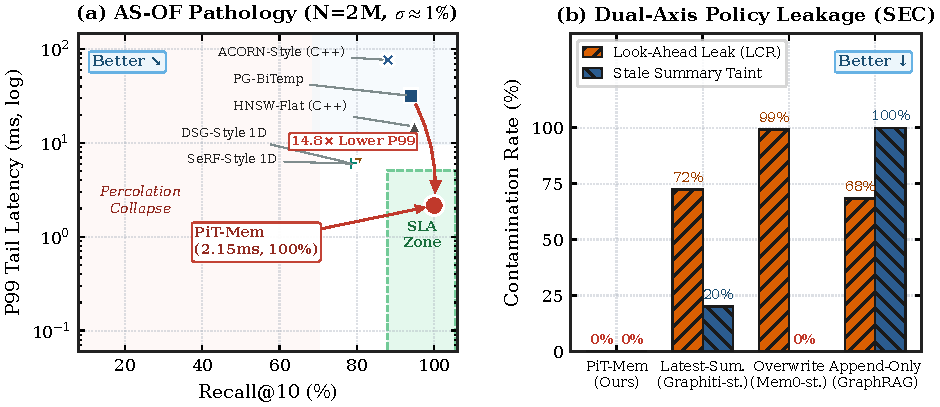
\includegraphics[width=\linewidth]{figures/fig1_motivation.pdf}
    \Description{Two-panel motivational chart showing P99 latency and recall degradation on narrow bi-temporal queries on the left, and bidirectional look-ahead vs stale reflection taint across surrogate memory policies on the right.}
    \caption{Motivating challenges on FinPiT-Bench: (a) narrow \texttt{AS OF} queries ($\sigma \approx 1\%$) stress \texttt{PG-BiTemp} tail latency and in-house post-filtered/1D graph adaptations; (b) unbranched summary policies exhibit bidirectional look-ahead and stale-taint leakage.}
    \label{fig:motivation}
\end{figure}

\subsection{Why Application-Layer Wrappers Struggle}

Recent temporal agent memory designs---such as Zep/\allowbreak Graphiti~\cite{rasmussen2025zep} and PostgreSQL bi-temporal GraphRAG (\texttt{post-graph-rag})~\cite{rajah2026postgraphrag}---attach four timestamps $(t_{\text{valid}},\allowbreak t_{\text{invalid}},\allowbreak t_{\text{created}},\allowbreak t_{\text{expired}})$ to property-graph edges or relational tuples backed by B-Trees and HNSW indexes~\cite{malkov2020hnsw, pgvector2024}. Yet Figure~\ref{fig:motivation} illustrates three core data-management bottlenecks when layering four timestamp columns atop general-purpose indexes:

\paragraph{Bottleneck 1: Four-Sided Mutable Interval Disconnection in Streaming ANNS\@.}
Point-in-Time semantic retrieval $Q(\mathbf{q}, t_v^*, t_k^*, k)$ requires Approximate Nearest Neighbor Search (ANNS) under a \emph{2D four-sided interval stabbing predicate}:
\[
t_v^s \le t_v^* < t_v^e \;\land\; t_k^s \le t_k^* < t_k^e.
\]
In global post-filtered proximity graphs~\cite{malkov2020hnsw} or predicate-agnostic 2-hop overlays~\cite{patel2024acorn}, chronologically arriving records insert reverse edges into older nodes' bounded neighbor lists and trigger degree pruning, progressively evicting historical peers. When replaying narrow historical windows ($\sigma \le 1.5\%$), $>98\%$ of graph neighbors fail the four-sided visibility check, stalling traversal across expired bridge nodes. Even in RAM-buffered PostgreSQL with \texttt{pgvector} v0.8~\cite{pgvector2024} and composite B-Trees, the executor faces an uncoupled access path between iterative HNSW expansion over dead heap tuples and B-Tree heap scans (Figure~\ref{fig:motivation}a). Meanwhile, 1D range-filtering ANNS indexes---SeRF~\cite{zuo2024serf}, UNIFY~\cite{liang2024unify}, and Dynamic Segment Graphs (DSG)~\cite{peng2025dsg}---index a \emph{single immutable scalar key}; they cannot natively prune 2D intervals whose right endpoints $(t_v^e, t_k^e)$ start at $+\infty$ and shrink in-place via \texttt{EVOLVE} and \texttt{RESTATE} commits.

\paragraph{Bottleneck 2: Reflection Contamination vs.\ Re-Consolidation Cost.}
Hierarchical memory consolidation---synthesizing episodic facts into reflection nodes or community summaries---is central to multi-hop agentic reasoning~\cite{park2023generative, li2026agenticmemory, rasmussen2025zep}. Versioning raw edges while updating entity summaries in-place leaks post-restatement knowledge into $t_k^* < t_k^{\text{restate}}$ ($\GraphitiLCR$ LCR for the unbranched summary policy in Figure~\ref{fig:motivation}b), whereas leaving summaries static pollutes post-restatement audits ($t_k^* \ge t_k^{\text{restate}}$). Conversely, eagerly invoking an LLM to re-summarize every ancestor reflection on every write degrades ingestion throughput, while naively unpacking tainted summaries on every read bloats downstream prompt tokens and can distort Top-$k$ ranking.

\paragraph{Bottleneck 3: Quantitative Erasure vs.\ Cold-Tier Lookup Overhead.}
Compacting cold episodes via lossy summarization or embedding pooling risks erasing exact numerical thresholds in non-medoid disclosures (e.g., \emph{``Consolidated Net Debt to EBITDA shall not exceed $3.50\times$''}). Conversely, offloading extracted tuples to external columnar files or separate relational indexes decouples structured slot filtering from compact semantic centroids, increasing cold-tier hybrid lookup overhead.

\begin{table*}[t]
\centering
\caption{Architectural comparison of PiT-Mem against representative agent memory, temporal graph, and filtered ANNS paradigms.}
\label{tab:comparison}
\small
\resizebox{\textwidth}{!}{%
\begin{tabular}{lcccccc}
\toprule
\textbf{System / Paradigm} & \textbf{Temporal Axes} & \textbf{Streaming 2D ANNS} & \textbf{Mutable Right-End} & \textbf{Provenance MVCC} & \textbf{Durability \& Cold Tier} \\
\midrule
Mem0~\cite{chhikara2025mem0} / Naive GraphRAG~\cite{edge2024graphrag} & None / Overwrite & Standard HNSW & Overwrite (Leaks) & None & Lossy LLM Summary \\
Zep / Graphiti~\cite{rasmussen2025zep} & 2D Schema Only & Post-Filter HNSW & Edge-Only Update & Unbranched Summary & Lossy Community Text \\
\texttt{post-graph-rag} (\texttt{pgvector})~\cite{rajah2026postgraphrag, pgvector2024} & 2D Relational & Iterative Heap / B-Tree & Heap Tuple MVCC & None & Disk Heap Pages \\
AeonG~\cite{hou2024aeong} & 1D Tx Time & No Vector ANNS & MVCC Anchor+Delta & Structural Graph Only & Delta Chain Storage \\
Filtered-DiskANN~\cite{gollapudi2023filtereddiskann} / ACORN~\cite{patel2024acorn} & Static Predicates & 2-Hop Predicate Graph & Degree-Diluted Filter & N/A & Static Index Snapshot \\
SeRF~\cite{zuo2024serf} / UNIFY~\cite{liang2024unify} / DSG~\cite{peng2025dsg} & 1D Static Scalar & 1D Segment Graph & Immutable Attr.\ Only & N/A & In-Memory Only \\
\midrule
\textbf{PiT-Mem (Ours)} & \textbf{2D Bi-Temporal} & \textbf{Causal Macro-Seg BiT-HNSW} & \textbf{$O(1)$ SoA Death-Tick} & \textbf{Re-Ranked Lazy-Branch} & \textbf{\texttt{mmap}+WAL \& RAP-Compact} \\
\bottomrule
\end{tabular}}
\end{table*}

\subsection{Summary of Contributions}

We design and implement \textbf{PiT-Mem}, a C++17 bi-temporal storage and indexing engine for look-ahead-free agentic memory (Table~\ref{tab:comparison}):
\begin{enumerate}
    \item \textbf{Causal Bi-Temporal Algebra (\S\ref{sec:model})}: A 7-tuple provenance model with SQL:2011-inspired \texttt{EVOLVE} and \texttt{RESTATE} operators preserving historical belief and truth while isolating historical-slice reflections from forward evolutions.
    \item \textbf{Streaming BiT-HNSW, Routing \& Tiering (\S\ref{sec:arch}--\S\ref{sec:bithnsw})}: Self-sealing \emph{Causal Macro-Segments} ($128\text{K}\!\to\!416\text{K}$) calibrated via a Vitter lag reservoir and $>20\%$ skew guard, 32-bit \emph{Dual-Budget Causal-Prefix Adjacency}, 64B-aligned SoA death-tick tables filtered via unsigned AVX2, POSIX \texttt{mmap} FP32 offload ($\CoreIndexBytesPerRec$~B/rec counted core arrays; $\CoreIndexRAMGiB$~GiB at $\MaxCorpusScale$), an analytical SIMD router pairing graph search with \texttt{maddubs} SQ8 scans, manifest-atomic snapshots, and CRC-32 WAL\@.
    \item \textbf{Phase-Fair MVCC (\S\ref{sec:mvcc}) \& RAP-Compact (\S\ref{sec:compact})}: Starvation-free cohort RW locks and zero-LLM write tainting paired with adaptive $k_{\text{fetch}}$-doubling FP32 re-ranking ($|\mathcal{O}| \le k$) and CAS hotness branching, plus range-normalized \emph{Slotted Segments} supporting unified hot+cold search (\texttt{query\_\allowbreak tiered\_\allowbreak pit}) over 56B anchors.
    \item \textbf{FinPiT-Bench \& Evaluation (\S\ref{sec:eval})}: Across $\UniqueSeedPassages$ seed passages scaled to $\MaxCorpusScale$ vectors, we evaluate Pareto frontiers, \texttt{mmap} offload, 12-thread stress, 3-hop bursts, dual-protocol audits, and cold compaction with explicit scope disclosures.
\end{enumerate}

\section{Data Model and Operator Algebra}
\label{sec:model}

\subsection{Bi-Temporal Provenance Memory Model}

We represent discrete timestamps in $\mathbb{T} = \mathbb{N}_0 \cup \{+\infty\}$ as unsigned 32-bit integers (\texttt{uint32\_t}) counting seconds since \texttt{1990-01-01\allowbreak T00:00:00Z}, with sentinel $\texttt{INF\_TICK} = 2^{32}-1$ (\texttt{0xFFFF\allowbreak FFFF}) denoting $+\infty$ ($136$~years at $1$-second resolution in $4$~bytes).

\begin{definition}[Bi-Temporal Causal Memory Unit]
\label{def:unit}
A memory unit in PiT-Mem is an immutable-identity 7-tuple:
\begin{equation}
    m_i = \langle \text{id}_i,\; \mathbf{v}_i,\; G_i,\; \tau_v(m_i),\; \tau_k(m_i),\; \text{tier}_i,\; \mathcal{P}_i \rangle
\end{equation}
where $\text{id}_i \in \mathbb{N}_0$ ($64$-bit \texttt{uint64\_t}) is a unique version ID; $\mathbf{v}_i \in \mathbb{R}^d$ is an $\ell_2$-normalized embedding; $G_i = (s, p, o, \mathcal{A})$ is the payload with typed numerical/anchor attributes $\mathcal{A}$; $\tau_v(m_i) = [t_v^s, t_v^e)$ ($t_v^s < t_v^e$) is the half-open \textbf{valid-time interval}; $\tau_k(m_i) = [t_k^s, t_k^e)$ ($t_k^s < t_k^e$) is the half-open \textbf{transaction-time interval}; $\text{tier}_i \in \{\textsc{Raw}, \textsc{Reflect}, \textsc{Compact}\}$ is the tier; and $\mathcal{P}_i \subset \mathbb{N}_0$ is the parent set ($\mathcal{P}_i = \emptyset$ iff $\text{tier}_i = \textsc{Raw}$), inducing an acyclic provenance DAG $\mathcal{G}_{\mathcal{P}}$.
\end{definition}

Geometrically, each version $m_i$ spans an axis-aligned rectangle $R(m_i) = [t_v^s(m_i), t_v^e(m_i)) \times [t_k^s(m_i), t_k^e(m_i)) \subset \mathbb{T}^2$. Open-ended assertions initialize $t_v^e = t_k^e = +\infty$ at commit time $t_k^s$ and shrink dynamically along either axis upon subsequent disclosures.

\begin{definition}[Point-in-Time Stabbing Snapshot \& Causal Cleanliness]
\label{def:stab}
Given state $\mathcal{M}$ and query point $(t_v^*, t_k^*) \in \mathbb{T}^2$, the bi-temporal stabbing snapshot is:
\begin{equation}
\label{eq:stab}
\mathcal{D}(t_v^*, t_k^*) = \{ m_i \in \mathcal{M} \mid t_v^s \le t_v^* < t_v^e \;\land\; t_k^s \le t_k^* < t_k^e \}.
\end{equation}
Let $\mathcal{P}^*(m_i)$ denote the reflexive transitive ancestor closure of $m_i$ in $\mathcal{G}_{\mathcal{P}}$. A retrieved result set $\mathcal{O} \subset \mathcal{D}(t_v^*, t_k^*)$ for $Q(\mathbf{q}, t_v^*, t_k^*, k)$ satisfies strict Point-in-Time isolation iff $|\mathcal{O}| \le k$ and:
\begin{enumerate}
    \item \textbf{Zero Look-Ahead Contamination ($\text{LCR} = 0$)}: Every $x \in \mathcal{O}$ and every ancestor $a \in \mathcal{P}^*(x)$ satisfies $t_k^s(a) \le t_k^*$.
    \item \textbf{Zero Post-Restatement Stale Taint ($\text{STR} = 0$)}: No $x \in \mathcal{O}$ has an ancestor $a \in \mathcal{P}^*(x)$ invalidated via \texttt{RESTATE} at $t_k^{\text{restate}} \le t_k^*$ over a valid interval overlapping $\tau_v(x)$.
\end{enumerate}
\end{definition}

\subsection{Operator Semantics: \texttt{EVOLVE} vs.\ \texttt{RESTATE}}

Conflating state evolution with retroactive restatement breaks bi-temporal auditability. Suppose an issuer's credit status is ingested on $t_k^0 = \text{Feb 1}$ as \texttt{Compliant} over $[\text{Jan 1}, +\infty) \times [\text{Feb 1}, +\infty)$, and on $t_k^{\text{now}} = \text{May 10}$ transitions to \texttt{Watchlist} effective $t_v^{\text{chg}} = \text{Apr 1}$. Mutating $t_v^e \leftarrow \text{Apr 1}$ in-place erases \texttt{Compliant} from a historical replay at $(\text{Apr 15}, \text{Apr 15})$, whereas closing only $t_k^e \leftarrow \text{May 10}$ loses Q1 compliance for a modern audit at $(\text{Feb 15}, \text{Jun 1})$. Extending SQL:2011 temporal semantics~\cite{snodgrass1999developing, kulkarni2012sql2011} to provenance DAGs, PiT-Mem defines three transactional operators:
\begin{enumerate}
    \item $\texttt{INSERT}(m_{\text{new}}, t_k^{\text{now}})$: Appends version $\text{id}_{\text{new}}$ with $t_k^s = t_k^{\text{now}}$, $t_k^e = +\infty$, and valid interval $[t_v^s, t_v^e)$.
    \item \texttt{EVOLVE}($m_{\text{old}}$, $m_{\text{new}}$, $t_v^{\text{chg}}$, $t_k^{\text{now}}$): Splits an active assertion ($t_k^e = +\infty$, $t_k^s < t_k^{\text{now}}$) at $t_v^{\text{chg}} \in (t_v^s, t_v^e)$ with $t_v^e(m_{\text{new}}) = t_v^e(m_{\text{old}})$:
    (a) close $t_k^e(m_{\text{old}}) \leftarrow t_k^{\text{now}}$ in $O(1)$;
    (b) insert continuation slice $m_{\text{hist}}$ cloning $(\mathbf{v}_{\text{old}}, G_{\text{old}})$ on $[t_v^s(m_{\text{old}}), t_v^{\text{chg}}) \times [t_k^{\text{now}}, +\infty)$ under a disjoint internal ID namespace;
    (c) insert evolved slice $m_{\text{new}}$ on $[t_v^{\text{chg}}, t_v^e(m_{\text{old}})) \times [t_k^{\text{now}}, +\infty)$; and
    (d) leave reflections scoped to $\tau_v(r) \subseteq [t_v^s(m_{\text{old}}), t_v^{\text{chg}})$ \textbf{untainted}, and attach an evolution watermark $(t_v^{\text{chg}}, t_k^{\text{now}})$ to overlapping reflections so queries at $t_v^* \ge t_v^{\text{chg}} \land t_k^* \ge t_k^{\text{now}}$ unpack updated evidence.
    \item $\texttt{RESTATE}(m_{\text{old}},\allowbreak m_{\text{new}},\allowbreak t_k^{\text{now}})$: Corrects an erroneous active assertion over $\tau_v(m_{\text{old}})$:
    (a) close $t_k^e(m_{\text{old}}) \leftarrow t_k^{\text{now}}$ in $O(1)$ without a continuation slice;
    (b) insert corrected $m_{\text{new}}$ on $\tau_v(m_{\text{old}}) \times [t_k^{\text{now}}, +\infty)$, inheriting reverse links $\mathcal{P}^{-1}$; and
    (c) traverse $\mathcal{P}^{-1*}(m_{\text{old}})$ unconditionally across intermediate ancestors to propagate taint watermark $t_k^{\text{susp}}(r) \leftarrow \min(t_k^{\text{susp}}(r),\allowbreak t_k^{\text{now}})$ and replacement $(m_{\text{old}} \to m_{\text{new}})$ to every active reflection $r$ with $\tau_v(r) \cap \tau_v(m_{\text{old}}) \neq \emptyset$ and $t_k^e(r) > t_k^{\text{now}}$.
\end{enumerate}

\begin{proposition}[Partition Completeness of Operators]
\label{prop:evolve}
For any attribute initialized at $[t_v^0, +\infty) \times [t_k^0, +\infty)$, any sequence of precondition-valid \texttt{EVOLVE} and \texttt{RESTATE} commits at strictly increasing $t_k^{(1)} < \dots < t_k^{(m)}$ on active versions ($t_k^e = +\infty$) partitions $[t_v^0, +\infty) \times [t_k^0, +\infty)$ into pairwise-disjoint rectangles $R(m_i) \cap R(m_j) = \emptyset$ ($i \neq j$) covering every $(t_v^*, t_k^*)$ uniquely.
\end{proposition}
\begin{proof}
By induction on $t_k^{(1)} < \dots < t_k^{(m)}$. Acting on active $R(m_{\text{old}}) = [a, b) \times [t_k^s, +\infty)$, \texttt{RESTATE} splits $R(m_{\text{old}})$ along $t_k = t_k^{\text{now}}$ into $[a, b) \times [t_k^s, t_k^{\text{now}})$ and $[a, b) \times [t_k^{\text{now}}, +\infty)$, while \texttt{EVOLVE} at $c \in (a, b)$ yields disjoint $[a, b) \times [t_k^s, t_k^{\text{now}})$, $[a, c) \times [t_k^{\text{now}}, +\infty)$, and $[c, b) \times [t_k^{\text{now}}, +\infty)$ whose union equals $R(m_{\text{old}})$.
\end{proof}

\section{System Architecture and Durability}
\label{sec:arch}

Figure~\ref{fig:arch} illustrates PiT-Mem's four-stage architecture, implemented in C++17 SIMD/OpenMP storage, indexing, MVCC, and persistence kernels exposed via zero-copy \texttt{pybind11} bindings.

\begin{figure*}[t]
    \centering
    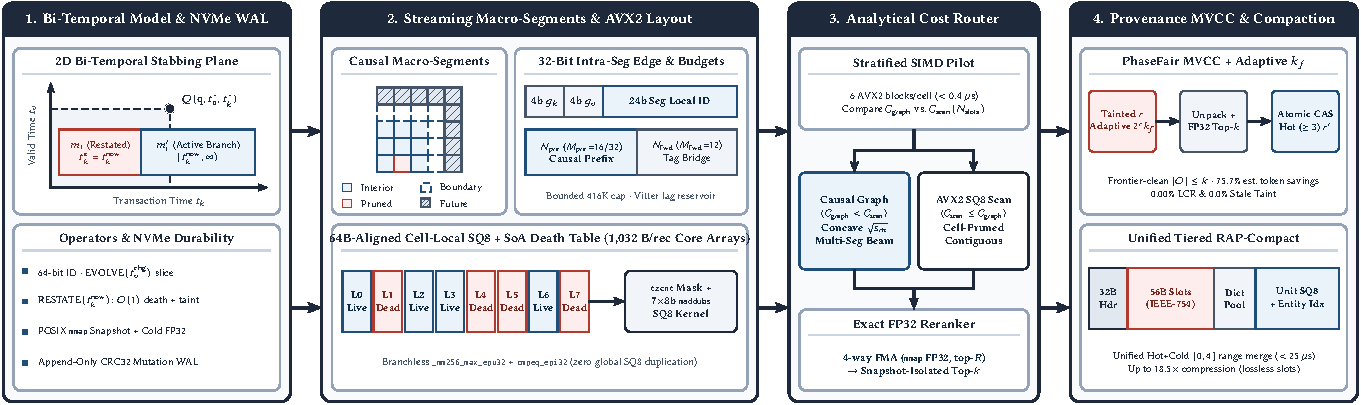
\includegraphics[width=0.90\textwidth]{figures/fig2_architecture.pdf}
    \Description{Four-swimlane system architecture and physical data layout blueprint of PiT-Mem across Bi-Temporal Algebra, BiT-HNSW Causal Macro-Segments, Analytical Cost Router, and Phase-Fair MVCC + Unified Tiered RAP-Compact.}
    \caption{Architecture and physical storage/index blueprint of PiT-Mem across four hardware-conscious execution stages.}
    \label{fig:arch}
\end{figure*}

\begin{table}[t]
\centering
\caption{Counted per-record index array layout of BiT-HNSW ($d = 768$, $M_{\text{pre}} = 16$ [$32$ intra-cell], $M_{\text{fwd}} = 12$). Auxiliary ID hash-map/allocator structures and file-backed OS page-cache residency are excluded from counted core-array bytes.}
\label{tab:mem_layout}
\small
\resizebox{\columnwidth}{!}{%
\begin{tabular}{llrr}
\toprule
\textbf{Buffer Component} & \textbf{Physical Encoding \& Tier} & \textbf{Bytes / Rec} & \textbf{Core Share} \\
\midrule
Cell-Local SQ8 + Meta & \texttt{int8[768]} + 12~B scale/norm/sum (RAM) & 780~B & $75.6\%$ \\
Dual-Budget + Hub Graph & $(32 + 12) \times \texttt{uint32\_t}$ + L1+ hubs (RAM) & 200~B & $19.4\%$ \\
64-Bit ID \& Slot Meta & \texttt{uint64} ID + cell/slot tags (RAM) & 20~B & $1.9\%$ \\
Segment + Cell SoA Ticks & $2 \times 4 \times \texttt{uint32\_t}$ (RAM) & 32~B & $3.1\%$ \\
\midrule
\textbf{Counted Core Arrays} & \textbf{Hot Search Arrays (\CoreIndexRAMGiB~GiB @ \MaxCorpusScale)} & \textbf{\CoreIndexBytesPerRec~B} & \textbf{$100.0\%$} \\
\midrule
Master Semantic Vector & 64B-aligned \texttt{float32[768]} (POSIX \texttt{mmap}) & 3{,}072~B & \emph{NVMe Paged} \\
\textbf{Total Counted Layout} & \textbf{Arrays + \texttt{mmap} (\PiTMemGiB~GiB All-RAM @ \MaxCorpusScale)} & \textbf{4{,}104~B} & --- \\
\bottomrule
\end{tabular}}
\end{table}

\paragraph{Single-Copy SQ8 Core Arrays \& POSIX \texttt{mmap} Cold-FP32 Offload.}
Table~\ref{tab:mem_layout} details BiT-HNSW's counted per-record index array hierarchy at $d = 768$. Each record stores a \emph{single canonical} 64B-aligned INT8 code vector inside its birth-epoch cell, shared by sequential cell scans and 1-hop graph evaluations via a compact \texttt{(cell\_id,\allowbreak slot\_idx)} handle. Because full $3{,}072$~B FP32 vectors are never touched during traversal or scanning---being gathered solely for final exact re-ranking of $R \ll N$ finalists---PiT-Mem provides \texttt{offload\_\allowbreak fp32\_\allowbreak to\_\allowbreak mmap}~\cite{leis2018leanstore, subramanya2019diskann}, flushing per-segment FP32 buffers to NVMe backing files mapped with \texttt{MADV\_\allowbreak RANDOM} and releasing anonymous heap arrays. This lowers \emph{counted core index-array footprint} from $4{,}104$~B/rec ($\PiTMemGiB$~GiB All-RAM) to \textbf{$\CoreIndexBytesPerRec$~B/rec} ($\CoreIndexRAMGiB$~GiB at $\MaxCorpusScale$), while process RSS additionally includes auxiliary ID hash maps and OS-cached FP32 pages.

\paragraph{NVMe Checkpointing \& Transactional CRC-32 WAL\@.}
PiT-Mem pairs manifest-atomic binary snapshots with a transactional WAL:
\begin{itemize}
    \item \textbf{Manifest-Atomic Checkpoints}: \texttt{save\_\allowbreak snapshot} persists generation-stamped \texttt{MacroSegment} CSR adjacency, SoA timestamps, mortality histograms, vectors (\texttt{"PITMSNP3"}), and DAG state (\texttt{"PITPROV2"}) via \texttt{fsync}, commits atomically by renaming a CRC-32 manifest (\texttt{"PITMANF1"}) with directory \texttt{fsync}, and restores segments via sequential \texttt{mmap} (\texttt{MADV\_\allowbreak SEQUENTIAL}).
    \item \textbf{Transactional CRC-32 WAL}: Online \texttt{INSERT}, \texttt{EVOLVE}, \texttt{RESTATE}, and branch commits append LSN-ordered frames (\texttt{"PWAL"} / \texttt{"PVWL"}) bracketed by \texttt{BEGIN\_TX} and \texttt{COMMIT\_TX}, guarded by IEEE~802.3 CRC-32 (\texttt{0xEDB88320}), and synced via \texttt{fdatasync}. On restart, \texttt{replay\_wal} skips frames up to $\mathrm{lsn}_{\text{ckpt}}$, checks CRCs, truncates torn or uncommitted tails, and replays committed mutations.
\end{itemize}

\section{BiT-HNSW: Streaming Mutable-Endpoint Hybrid Indexing}
\label{sec:bithnsw}

\subsection{Disconnection of Post-Filtered Graphs}

Consider $N$ versions arriving in transaction order $t_k(m_1) \le \dots \le t_k(m_N)$ with uniform embeddings on $\mathbb{S}^{d-1}$. In a global $2M$-bounded proximity graph, inserting later nodes $j > i$ adds reverse edges $(u \to j)$ into historical node $u$'s neighbor list and triggers heuristic pruning once $|\mathcal{N}(u)| > 2M$.

\begin{proposition}[Expected Visible Degree Collapse]
\label{prop:collapse}
Under a uniform $2M$-regular neighborhood model where chronological neighbor replacement and right-endpoint survival act independently of embedding proximity, for a historical query $(t_v^*, t_k^*)$ with birth selectivity $\sigma_{\text{birth}}$ and conditional survival rate $\rho_{\text{surv}}$ ($\sigma = \sigma_{\text{birth}} \rho_{\text{surv}}$), the expected visible degree of $u \in \mathcal{D}(t_v^*, t_k^*)$ is $\mathbb{E}[|\mathcal{N}(u) \cap \mathcal{D}(t_v^*, t_k^*)|] = 2M \cdot \sigma$. Whenever $\sigma < \frac{1}{2M}$ (e.g., $\sigma = 0.01, M = 16 \implies \mathbb{E}[\deg_{\text{vis}}] = 0.32 < 1$), the visible induced subgraph $\mathcal{G}[\mathcal{D}(t_v^*, t_k^*)]$ falls below the giant-component percolation threshold.
\end{proposition}

Predicate-agnostic 2-hop overlays~\cite{patel2024acorn} inspect $\Theta(M^2)$ two-hop neighbors per step, mitigating moderate filtering ($\sigma \ge 20\%$) at higher check cost, while 1D segment graphs~\cite{zuo2024serf, peng2025dsg} order records by a single immutable scalar attribute and cannot prune the second birth axis or dynamically shrinking right endpoints $(t_v^e, t_k^e)$.

\subsection{Streaming-Native Causal Macro-Segments \& Dual-Budget Adjacency}

BiT-HNSW exploits the \emph{asymmetry of mutability} in bi-temporal streams: right endpoints $t_v^e$ and $t_k^e$ shrink unpredictably in place, whereas \textbf{birth coordinates $(t_v^s, t_k^s)$ are immutable at creation}. An online engine cannot rely on offline future quantiles or freeze a bootstrap grid without boundary-cell pile-up.

\paragraph{Bounded Causal Macro-Segments \& Vitter Lag Calibration.}
BiT-HNSW partitions an unbounded 64-bit stream into self-sealing \textbf{Causal Macro-Segments} $\mathcal{S}_0, \dots, \mathcal{S}_m$ with capacities $C_0 = 128\text{K}$, $C_1 = 256\text{K}$, $C_m = C_{\max} = 416\text{K} < 2^{24}$ for $m \ge 2$ (mapping 64-bit IDs to $(\texttt{seg\_id} \ll 32) \mid \texttt{local\_id}$):
\begin{enumerate}
    \item \textbf{Online Row-Budget Transaction Epochs ($g_k \in [0, B-1]$)}: Because $t_k^s$ arrives monotonically, each $\mathcal{S}_m$ advances column $g_k$ online at $\lceil C_m / B \rceil$ arrivals ($B = 16$), recording bounds $[t_{k,\min}^s[g_k],\allowbreak t_{k,\max}^s[g_k]]$ with zero future knowledge.
    \item \textbf{Vitter Lag-Convolution Quantiles ($g_v \in [0, B-1]$) \& Skew Guard}: PiT-Mem maintains a $4{,}096$-sample \textbf{Vitter reservoir}~\cite{vitter1985reservoir} of observed lags $\Delta_j = \max(0, t_k^s(j) - t_v^s(j))$. Sealing $\mathcal{S}_{m-1}$ at $t_k^{(0)}$ with scaled span $\widehat{\Delta T}_k$ (proportional to $C_m / |\mathcal{S}_{m-1}|$), $\mathcal{S}_m$'s $B-1$ valid-time ticks use empirical $\frac{b}{B}$-quantiles of $t_k^{(0)} + u_q \widehat{\Delta T}_k - \Delta_j$ ($u_q \in \{0.03,\dots,0.97\}$). An \textbf{all-bin skew guard} seals $\mathcal{S}_m$ early whenever any $g_v$ bin exceeds $20\%$ of $C_m$ after $8{,}192$ arrivals, preventing both $(15,15)$ pile-up and interior skew without rewiring.
\end{enumerate}
Within each segment, the $B \times B = 256$ cells $C_{g_v, g_k}$ classify query $(t_v^*, t_k^*)$ with bin $(q_v, q_k)$ into \emph{Future Cells} (pruned in $O(1)$), \emph{Interior Fully-Born Cells} ($t_{v,\max}^s \le t_v^* \land t_{k,\max}^s \le t_k^*$, reducing checks to 2-sided death filtering), and \emph{Boundary Cells} (4-sided checks).

\paragraph{Dual-Budget Adjacency \& Epoch Tags.}
Each \texttt{MacroSegment} maintains a Layer-1 causal hub overlay (sampled at $1/16$ with disjoint visited tokens) atop a Layer-0 graph splitting each node $u$'s adjacency into two budgets:
\begin{itemize}
    \item \textbf{Causal-Prefix List $\mathcal{N}_{\text{pre}}(u)$ ($M_{\text{pre}} = 16$ outgoing, $2M_{\text{pre}} = 32$ intra-cell cap)}: RNG-diversified neighbors $w$ in the causal prefix $g_v(w) \le g_v(u) \land g_k(w) \le g_k(u)$, barring reverse edges from later cells.
    \item \textbf{Forward-Bridge List $\mathcal{N}_{\text{fwd}}(u)$ ($M_{\text{fwd}} = 12$)}: Absorbs reverse edges $(u \to z)$ from strictly later cells ($g_v(z) > g_v(u) \lor g_k(z) > g_k(u)$) for broad-window upward navigation.
\end{itemize}
Each intra-segment neighbor word packs 8-bit birth coordinates alongside the 24-bit segment-local ID:
\[
\texttt{packed} = (\texttt{gk} \ll 28) \mid (\texttt{gv} \ll 24) \mid (\texttt{local\_id} \;\&\; \texttt{0xFFFFFF}).
\]
During traversal at $(q_v, q_k)$, out-of-snapshot entries in $\mathcal{N}_{\text{fwd}}(u)$ are rejected via ALU shifts in L1 cache without dereferencing target vectors or timestamps.

\begin{theorem}[Causal-Prefix Subgraph Invariance]
\label{thm:prefix}
Within any \texttt{MacroSegment} $\mathcal{S}_m$, for any query bin $(q_v, q_k) \in \{0, \dots, B-1\}^2$ and any subsequent insertions into later cells $(g_v, g_k) \notin [0..q_v] \times [0..q_k]$ or later segments $\mathcal{S}_{m'}$ ($m' > m$), the prefix-restricted causal subgraph $\mathcal{G}_{\text{pre}}[V_{\le (q_v, q_k)}]$ is strictly invariant: every $u \in V_{\le (q_v, q_k)}$ retains $100\%$ of $\mathcal{N}_{\text{pre}}(u) \subseteq V_{\le (q_v, q_k)}$, and out-of-prefix entries in $\mathcal{N}_{\text{fwd}}(u)$ are rejected in registers without dereferences outside $V_{\le (q_v, q_k)}$.
\end{theorem}
\begin{proof}
Insertions into $\mathcal{S}_{m'}$ ($m' > m$) never touch $\mathcal{S}_m$. Within $\mathcal{S}_m$, any later-cell node $z$ with $g_v(z) > q_v$ or $g_k(z) > q_k$ routes reverse edges $(u \to z)$ exclusively to $\mathcal{N}_{\text{fwd}}(u)$, leaving $\mathcal{N}_{\text{pre}}(u)$ immutable once cell $(g_v(u), g_k(u))$ seals; inline tags $(\texttt{gv}(z), \texttt{gk}(z))$ filter $\mathcal{N}_{\text{fwd}}(u)$ before any target load.
\end{proof}
At $10^8+$ scale, asynchronous LSM-style segment merging or automatic cold-tier demotion to bound cross-segment fan-out remains future work beyond our $2\text{M}$-scale evaluation.

\subsection{SoA Death-Tick Tables \& Non-Saturating AVX2 Kernels}

Right-endpoint updates under \texttt{EVOLVE} and \texttt{RESTATE} never rewire graph edges. Each cell stores four 64B-aligned SoA \texttt{uint32\_t} arrays (\texttt{tv\_s[]}, \texttt{tv\_e[]}, \texttt{tk\_s[]}, \texttt{tk\_e[]}) padded to multiples of 8, updating closures and mortality histograms in $O(1)$.

\paragraph{Unsigned AVX2 Stabbing.}
Because x86 AVX2 \texttt{\_mm256\_\allowbreak cmpgt\_\allowbreak epi32} is signed, sentinel $t^e = \texttt{0xFFFF\allowbreak FFFF}$ ($-1$ signed) would be misclassified as $-1 < t^*$. Exploiting $a < b \iff \max_u(a, b) \neq a$, BiT-HNSW evaluates 2-sided interior checks ($t_v^* < t_v^e \land t_k^* < t_k^e$) across 8 records in 6 branchless SIMD instructions (\texttt{\_mm256\_\allowbreak max\_\allowbreak epu32}, \texttt{cmpeq\_\allowbreak epi32}, \texttt{or\_\allowbreak si256}, \texttt{movemask\_\allowbreak ps}) and 4-sided boundary checks in 11 instructions, iterating surviving lanes via \texttt{\_\_builtin\_\allowbreak ctz}.

\paragraph{Non-Saturating Biased-7$\times$8-Bit \texttt{maddubs} SQ8.}
Each vector $\mathbf{x}_i$ is quantized into symmetric INT8 codes $x_{i,j}^{\text{s8}} = \text{round}(x_{i,j}/\alpha_i) \in [-127, 127]$ ($\alpha_i = \|\mathbf{x}_i\|_\infty / 127$) with precomputed $\|\mathbf{x}_i\|_2^2$ and $S_i = \sum_{j=1}^d x_{i,j}^{\text{s8}}$.

\begin{proposition}[Non-Saturating \texttt{maddubs} Bound]
\label{prop:sq8}
Quantizing query coordinates with $\alpha_q = \|\mathbf{q}\|_\infty / 63$ into biased 7-bit unsigned integers $u_j = \text{round}(q_j / \alpha_q) + 64 \in [1, 127]$ ensures $|u_{2m} x_{i,2m}^{\text{s8}} + u_{2m+1} x_{i,2m+1}^{\text{s8}}| \le 2 \times 127^2 = 32{,}258 \le 32{,}767$, preventing signed \texttt{int16\_t} saturation in \texttt{\_mm256\_\allowbreak maddubs\_\allowbreak epi16}. The inner product $\langle \hat{\mathbf{q}}, \hat{\mathbf{x}}_i \rangle$ equals $\alpha_q \alpha_i (\sum_j u_j x_{i,j}^{\text{s8}} - 64 S_i)$, with per-coordinate error at most $\frac{|q_j|\alpha_i + |x_{i,j}|\alpha_q}{2} + \frac{\alpha_q \alpha_i}{4}$.
\end{proposition}
Exact 4-way AVX2 FMA FP32 re-ranking over a top-$R$ SQ8 finalist pool, with $R = \max(8k, \min(3ef, 1{,}536))$ ($R = \max(6k, 64)$ on the scan path), reduces quantization distortion while keeping approximate-search candidate bounds explicit.

\begin{algorithm}[t]
\caption{BiT-HNSW Analytical Multi-Segment Hybrid Search}
\label{alg:search}
\footnotesize
\begin{algorithmic}[1]
\Require Query $(\mathbf{q}, t_v^*, t_k^*, k, ef)$, Causal Macro-Segments $\{\mathcal{S}_m\}$
\Ensure Snapshot-visible approximate top-$k$ list $\mathcal{R}$
\State $\mathcal{Q}_{\text{cells}} \gets \emptyset$; $N_{\text{slots}}, \hat{N}_{\text{born}}, \hat{N}_{\text{alive}} \gets 0$; $ef_{\max} \gets \max(ef, 2k)$; $ef_{\min} \gets \min(ef_{\max}, \max(3k, 32))$
\For{each $\mathcal{S}_m$ with $\text{min\_tv\_s} \le t_v^* \land \text{min\_tk\_s} \le t_k^*$}
    \State $(q_v, q_k) \gets (\text{Bin}_v(\mathcal{S}_m, t_v^*),\; \text{Bin}_k(\mathcal{S}_m, t_k^*))$; accumulate $\hat{b}_m$ into $\hat{N}_{\text{born}}$; \textbf{if} $\text{max\_tv\_e} \le t_v^* \lor \text{max\_tk\_e} \le t_k^*$ \textbf{continue}
    \For{$g_k = 0 \dots q_k$ (if $k_{\min}[g_k] \le t_k^*$) \textbf{and} $g_v = 0 \dots q_v$}
        \State $C \gets \mathcal{S}_m.C_{g_v, g_k}$; \textbf{if} bbox or mortality tail $\sum H_{v/k} = 0$ \textbf{continue}
        \State $\text{fb} \gets \text{isFullyBorn}(C, t_v^*, t_k^*)$; append $(\mathcal{S}_m, C, \text{fb})$ to $\mathcal{Q}_{\text{cells}}$; $N_{\text{slots}} \mathrel{+}= |C|$
        \State $\hat{a}_C \gets \text{StratifiedSIMDPilot6}(C, \text{fb}, t_v^*, t_k^*)$; accumulate $\hat{a}_m, \hat{N}_{\text{alive}}$
    \EndFor
\EndFor
\State $\mathbf{q}_{\text{sq8}} \gets \text{QuantizeQueryU7}(\mathbf{q})$; $R \gets \max(8k, \min(3ef, 1{,}536))$; $\mathcal{C}_{\text{fin}} \gets \emptyset$
\State Evaluate $\mathcal{C}_{\text{scan}}(N_{\text{slots}}, \hat{N}_{\text{alive}})$ and $\mathcal{C}_{\text{graph}}(\{(\hat{b}_m, \hat{a}_m)\})$ via Eq.~\eqref{eq:router}
\If{$\hat{\rho} \ge \rho_{\min} \;\land\; \mathcal{C}_{\text{graph}} < 0.92\,\mathcal{C}_{\text{scan}}$} \Comment{Causal Graph Path}
    \For{qualifying $\mathcal{S}_m$ ordered largest-$\hat{a}_m$-first ($s_m \gets \hat{a}_m / \hat{N}_{\text{alive}}$)}
        \If{$m > 0 \;\land\; \mathcal{C}_{\text{scan}}^{(m)} \le \mathcal{C}_{\text{graph}}^{(m)}$} scan $\mathcal{S}_m$ cells into top-$R$ $\mathcal{C}_{\text{fin}}$
        \Else
            \State $ef_m \gets (m\!=\!0) ? ef_{\max} : \text{clamp}(\lceil ef\max(0.55,\sqrt{s_m})\rceil,$ $\allowbreak ef_{\min}, ef_{\max})$; traverse $\mathcal{S}_m$ into $\mathcal{C}_{\text{fin}}$
        \EndIf
    \EndFor
\Else \Comment{Cell-Pruned AVX2 SQ8 Scan Path}
    \State $R \gets \max(6k, 64)$
    \For{$(\mathcal{S}_m, C, \text{fb}) \in \mathcal{Q}_{\text{cells}}$ \textbf{and} $\text{slot} = 0, 8, \dots, |C|-1$}
        \State $\text{mask} \gets \text{fb} \ ? \ \text{AVX2Death8}(C, \text{slot}) : \text{AVX2Full8}(C, \text{slot})$
        \For{set bit $b$ in $\text{mask}$} update top-$R$ heap $\mathcal{C}_{\text{fin}}$ via $C.\text{sq8}[\text{slot}+b]$ \EndFor
    \EndFor
\EndIf
\State \Return $\text{ExactFP32Rerank}(\mathbf{q}, \mathcal{C}_{\text{fin}}, k)$ \Comment{Reads RAM or \texttt{mmap} FP32}
\end{algorithmic}
\end{algorithm}

\subsection{Mortality Pruning \& Analytical Multi-Segment Cost Router}

Each cell maintains death maxima $(\text{max\_tv\_e},\allowbreak \text{max\_tk\_e})$ and two 16-bin mortality histograms $H_v, H_k$ (bin $15$ tracks \texttt{INF\_TICK}), pruning dead cells in $O(1)$. Across surviving cells ($N_{\text{slots}}$ slots), a stratified 6-block SIMD pilot (\texttt{StratifiedSIMDPilot6}) probes up to $6$ strided 8-slot AVX2 blocks/cell to estimate $\hat{a}_m$ and $\hat{N}_{\text{alive}} = \sum_m \hat{a}_m$, evaluating an \textbf{analytical cost model} normalized to one $768$-d \texttt{maddubs} distance:
\begin{equation}
\label{eq:router}
\begin{aligned}
\mathcal{C}_{\text{scan}} &= \gamma_0 + \gamma_{\text{ts}} \frac{N_{\text{slots}}}{8} + \frac{d}{768}\,\hat{N}_{\text{alive}}, \\
\mathcal{C}_{\text{graph}} &= \sum_{m \in \mathcal{S}_{\text{qual}}} \!\min\!\Bigl(\mathcal{C}_{\text{scan}}^{(m)},\; \eta_{\text{mem}}(N)\Bigl[\gamma_{\text{hub}} + \frac{ef_m (\gamma_{\text{llc}} + \gamma_{\text{dim}}\frac{d}{768})}{\max(0.025, \hat{\rho}_m)^{0.80}}\Bigr]\Bigr),
\end{aligned}
\end{equation}
where $\hat{\rho}_m = \hat{a}_m / \max(1, \hat{b}_m)$, $\eta_{\text{mem}}(N) = \text{clamp}(N / 450{,}000,\allowbreak 0.24,\allowbreak 1.0)$ models the LLC-to-DRAM shift, and $(\gamma_0, \gamma_{\text{ts}}, \gamma_{\text{hub}}, \gamma_{\text{llc}}, \gamma_{\text{dim}})$ defaults to $(140, 0.125, 1{,}050, 6.25, 10.8)$ (startup-calibrated). Secondary segments use concave beam $ef_m$, clamping $\lceil ef \max(0.55, \sqrt{s_m}) \rceil$ to $[ef_{\min}, ef_{\max}]$ for share $s_m = \hat{a}_m / \hat{N}_{\text{alive}}$. Routing to the graph iff $\hat{\rho} = \hat{N}_{\text{alive}} / \hat{N}_{\text{born}} \ge 0.055$ and $\mathcal{C}_{\text{graph}} < 0.92\,\mathcal{C}_{\text{scan}}$ avoids routing inversion across sparse audits while accelerating moderate-to-broad snapshots.

\begin{theorem}[Bounded Sparse-Scan Query Complexity]
\label{thm:cost}
Across $M_{\text{seg}} = O(\log(\min(N, C_{\max}) / C_0) + N / C_{\max})$ macro-segments with $N_{\text{slots}}$ slots in non-pruned cells and $N_{\text{alive}}$ visible records, the scan branch of Algorithm~\ref{alg:search} executes $O(M_{\text{seg}} B^2 + N_{\text{slots}}/8 + N_{\text{alive}} d / 32 + R d / 8)$ SIMD operations and $O(N_{\text{alive}} \log R)$ heap updates, independent of future cells and sealed future segments.
\end{theorem}
\begin{proof}
Headers prune future segments, future cells, and dead cells in $O(M_{\text{seg}} B^2)$; surviving cells run $N_{\text{slots}}/8$ AVX2 filters, $N_{\text{alive}}$ 32-wide \texttt{maddubs} kernels, and $R$ 8-wide FMA dot products.
\end{proof}

\section{Phase-Fair Lazy-Branch MVCC for Provenance DAGs}
\label{sec:mvcc}

\subsection{Phase-Fair Concurrency \& Zero-LLM Taint Propagation}

An agent periodically consolidates supporting memories $\mathcal{P}_r$ into a \textsc{Reflect} summary $r$ over valid scope $\tau_v(r)$, enforcing $t_k^s(r) \ge \max_{p \in \mathcal{P}_r} t_k^s(p)$. Standard reader-preferring locks (\texttt{std::\allowbreak shared\_\allowbreak mutex}) allow sustained readers to starve streaming \texttt{RESTATE} commits or segment rollovers. PiT-Mem coordinates readers and writers via a C++17 \textbf{\texttt{PhaseFair\allowbreak SharedMutex}}~\cite{brandenburg2010phasefair} paired with per-reflection atomics~\cite{larson2011hekaton, neumann2015hyper, wu2017mvcc}: tainted-read counter $\text{hot}(r)$ and 3-state status $\text{state}(r) \in \{0, 1, 2\}$.

On creation, $r$ computes its transitive closure $\mathcal{P}^*(r)$~\cite{green2007provenance}, inherits overlapping ancestor watermarks, and subscribes to active slices; \texttt{EVOLVE} transfers interval-overlapping $\mathcal{P}^{-1}$ links onto $(m_{\text{hist}}, m_{\text{new}})$ while leaving historical slices untainted. When \texttt{RESTATE}($m_{\text{old}}$, $m_{\text{new}}$, $t_k^{\text{now}}$) commits: (1) BiT-HNSW closes $t_k^e(m_{\text{old}}) \leftarrow t_k^{\text{now}}$ in $O(1)$, inserts $m_{\text{new}}$ on $[t_k^{\text{now}}, +\infty)$, and copies $\mathcal{P}^{-1}$ subscriptions; and (2) unconditional reverse-DAG BFS marks every reachable active reflection $r$ ($t_k^e(r) > t_k^{\text{now}}$, $\tau_v(r) \cap \tau_v(m_{\text{old}}) \neq \emptyset$) with $t_k^{\text{susp}}(r) \leftarrow \min(t_k^{\text{susp}}(r), t_k^{\text{now}})$ and replacement $(m_{\text{old}} \to m_{\text{new}})$, executing zero LLM calls on the write path.

\begin{algorithm}[t]
\caption{Phase-Fair Adaptive Lazy-Branch MVCC Snapshot Read}
\label{alg:mvcc}
\footnotesize
\begin{algorithmic}[1]
\Require Query $(\mathbf{q}, t_v^*, t_k^*, k, ef)$, Hotness threshold $\theta_{\text{hot}}$
\Ensure Clean exact-re-ranked Top-$k$ context $\mathcal{O}$ ($|\mathcal{O}| \le k$)
\State Acquire shared reader phase on \texttt{PhaseFairSharedMutex}
\State $k_{\text{fetch}} \gets \max(2k, k + 12)$; $k_{\max} \gets \max(32k, 512)$; $r \gets 0$
\Repeat
    \State $\mathcal{C} \gets \text{BiTHNSW.Search}(\mathbf{q}, t_v^*, t_k^*, k_{\text{fetch}}, \max(ef, 2k_{\text{fetch}}))$
    \State $\mathcal{S}_{\text{pool}} \gets \emptyset$; $d_{\text{front}} \gets \max_{(m, d_m) \in \mathcal{C}} d_m$; $\text{anyTaint} \gets \textbf{false}$
    \For{each $(m, d_m) \in \mathcal{C}$}
        \If{$m.\text{tier} = \textsc{Reflect} \;\land\; m.\text{isTaintedAt}(t_v^*, t_k^*)$}
            \State $\text{anyTaint} \gets \textbf{true}$; \textbf{if} $r = 0 \land \text{rank}(m) < k$ \textbf{then} $\mathcal{D}_{\text{hit}} \gets \mathcal{D}_{\text{hit}} \cup \{m\}$
            \For{clean deduplicated $u \in \text{UnpackClean}(m, t_v^*, t_k^*)$}
                \State $\mathcal{L}[u] \gets \mathcal{L}[u] \cup \{m\}$; $\mathcal{S}_{\text{pool}} \gets \mathcal{S}_{\text{pool}} \cup \{(u,\; \|\mathbf{q} - \mathbf{v}_u\|_2^2)\}$
            \EndFor
        \ElsIf{$m$ not yet in $\mathcal{S}_{\text{pool}}$}
            \State $\mathcal{S}_{\text{pool}} \gets \mathcal{S}_{\text{pool}} \cup \{(m, d_m)\}$
        \EndIf
    \EndFor
    \State $n_{\le \text{front}} \gets |\{(x, d_x) \in \mathcal{S}_{\text{pool}} : d_x \le d_{\text{front}}\}|$; $r \gets r + 1$
    \If{$\neg\text{anyTaint} \;\lor\; n_{\le \text{front}} \ge k \;\lor\; |\mathcal{C}| < k_{\text{fetch}} \;\lor\; k_{\text{fetch}} \ge k_{\max}$} \textbf{break} \EndIf
    \State $k_{\text{fetch}} \gets \min(2 k_{\text{fetch}}, k_{\max})$ \Comment{Adaptive geometric doubling}
\Until{\textbf{false}}
\State $\mathcal{O} \gets \text{PartialSortTopK}(\mathcal{S}_{\text{pool}}, k)$ \Comment{Strictly enforces $|\mathcal{O}| \le k$}
\For{$m \in \mathcal{D}_{\text{hit}} \cup \bigcup_{u \in \mathcal{O}} \mathcal{L}[u]$ \textbf{with} $\text{atomic\_load}(m.\text{state}) = 0$}
    \If{$\text{atomic\_fetch\_add}(m.\text{hot}, 1) + 1 \ge \theta_{\text{hot}} \;\land\; \text{CAS}(m.\text{state}, 0 \to 1)$} EnqueueRepair($m$) \EndIf
\EndFor
\State \Return $\mathcal{O}$
\end{algorithmic}
\end{algorithm}

\subsection{Adaptive $k_{\text{fetch}}$-Doubling Unpack \& Non-Retroactive Branching}

Naive unpacking starves rank-$(k_{\text{fetch}}+1)$ clean candidates during clustered bursts, violates $|\mathcal{O}| \le k$, or schedules duplicate repair jobs under shared locks. Algorithm~\ref{alg:mvcc} resolves all three:
\begin{itemize}
    \item \textbf{Adaptive $k_{\text{fetch}}$ Doubling \& FP32 Re-Ranking}: Starting at $k_{\text{fetch}} = \max(2k,\allowbreak k+12)$, whenever $m$ is tainted, \texttt{UnpackClean} resolves multi-hop replacement chains and \texttt{EVOLVE} slices with $t_k^s \le t_k^*$, re-scores leaves via exact AVX2 FP32 distances $\|\mathbf{q} - \mathbf{v}_u\|_2^2$, and checks $|\{(x, d_x) \in \mathcal{S}_{\text{pool}} : d_x \le d_{\text{front}}\}| \ge k$. Uncontaminated reads finish in round $r=0$, while bursts double $k_{\text{fetch}}$ until $k$ clean items beat $d_{\text{front}}$.
    \item \textbf{CAS Scheduling \& Non-Retroactive Branching}: Readers increment $\text{hot}(m)$ only for tainted reflections affecting Top-$k$ and claim repair via $\text{CAS}(0 \to 1)$. At commit $t_k^{\text{mat}} \ge \max(t_k^{\text{susp}}(m),\allowbreak \max_{p \in \mathcal{P}_{m'}} t_k^s(p))$, the worker closes $t_k^e(m) \leftarrow t_k^{\text{mat}}$, stores $\text{state}(m) \leftarrow 2$, and inserts repaired $m'$ on $[t_k^{\text{mat}}, +\infty)$ without backdating $t_k^s(m')$.
\end{itemize}

\begin{theorem}[Snapshot Isolation \& Clean Completeness]
\label{thm:isolation}
For any sequence of precondition-valid \texttt{INSERT}, \texttt{EVOLVE}, \texttt{RESTATE}, and non-retroactive branch commits, Algorithm~\ref{alg:mvcc} returns $\mathcal{O}$ satisfying $|\mathcal{O}| \le k$, $\text{LCR} = 0$, and $\text{STR} = 0$ (Definition~\ref{def:stab}). Whenever the underlying search returns exact snapshot top-$k_{\text{fetch}}$ up to $d_{\text{front}}$ and exits with $n_{\le \text{front}} \ge k$ or $|\mathcal{C}| < k_{\text{fetch}}$, $\mathcal{O}$ equals the exact clean snapshot Top-$k$.
\end{theorem}
\begin{proof}
\texttt{PartialSortTopK} bounds $|\mathcal{O}| \le k$. Every $x \in \mathcal{O}$ passes \texttt{bitemp\_visible} and $\neg\text{isTaintedAt}$. By induction on DAG height, non-retroactive birth $t_k^s(r) \ge \max_{p \in \mathcal{P}_r} t_k^s(p)$ ensures $t_k^s(a) \le t_k^*$ for all $a \in \mathcal{P}^*(x)$ ($\text{LCR}=0$), while transitive watermark inheritance and unconditional reverse-BFS prevent overlapping restated ancestors ($\text{STR}=0$). If $\mathcal{C}$ covers all snapshot-visible items within $d_{\text{front}}$, any uninspected clean item has distance $\ge d_{\text{front}}$, so $n_{\le \text{front}} \ge k$ (or $|\mathcal{C}| < k_{\text{fetch}}$) certifies exact clean Top-$k$.
\end{proof}

\section{RAP-Compact \& Unified Hot-Cold Tiered Retrieval}
\label{sec:compact}

To bound cold-tier storage while preserving extracted quantitative assertions alongside semantic centroids, \textbf{RAP-Compact} packs structured tuples into a self-contained binary \textbf{Anchor-Residual Slotted Segment} (\texttt{"PIT3"}):
\begin{enumerate}
    \item \textbf{Schema-Parameterized Anchor Extraction}: Declarative grammars extract typed entity-metric-threshold tuples across credit covenants (Net Debt/EBITDA, Interest Coverage, Minimum Liquidity, comparators, and cure/cross-default/MAC flags) and GAAP XBRL items (Revenue, Net Income, Operating Income, Total Assets, EPS) with unit normalization.
    \item \textbf{Slotted Layout \& $[0, 4]$ Scoring}: Cold batches cluster passages within overlapping epochs into a contiguous segment storing: (a) a 32B \texttt{SlottedPageHeader}; (b) a 2B string dictionary; (c) 56B \texttt{PackedAnchorTuple} records (IEEE-754 \texttt{double} thresholds, unit/polarity tags, four \texttt{uint32\_t} ticks, and \texttt{cluster\_id}); and (d) 28B \texttt{PackedMemberSpan} descriptors (64-bit \texttt{source\_mem\_id}, bounds, snippet offsets). Both $d_{\text{sub}}$-d centroids $\bar{\mathbf{c}}$ and query prefixes $\tilde{\mathbf{q}}$ are $\ell_2$-normalized so cold SQ8 scores $\|\tilde{\mathbf{q}} - \bar{\mathbf{c}}\|_2^2 \in [0, 4]$ share the range of hot squared-$L_2$ distances (while remaining distinct approximate metrics vs.\ full-$d$ hot vectors).
    \item \textbf{Unified Hot+Cold Search (\texttt{query\_tiered\_pit})}: Given snapshot $(t_v^*, t_k^*)$, this operator searches hot \texttt{BiT-HNSW} and cold \texttt{RAP-Compact}, suppresses post-compaction cold retractions via an overlay map, deduplicates member IDs, merges candidates on $[0, 4]$ into Top-$k$, and returns matching 56B anchors.
\end{enumerate}

\section{Experimental Evaluation}
\label{sec:eval}

\begin{figure*}[t]
    \centering
    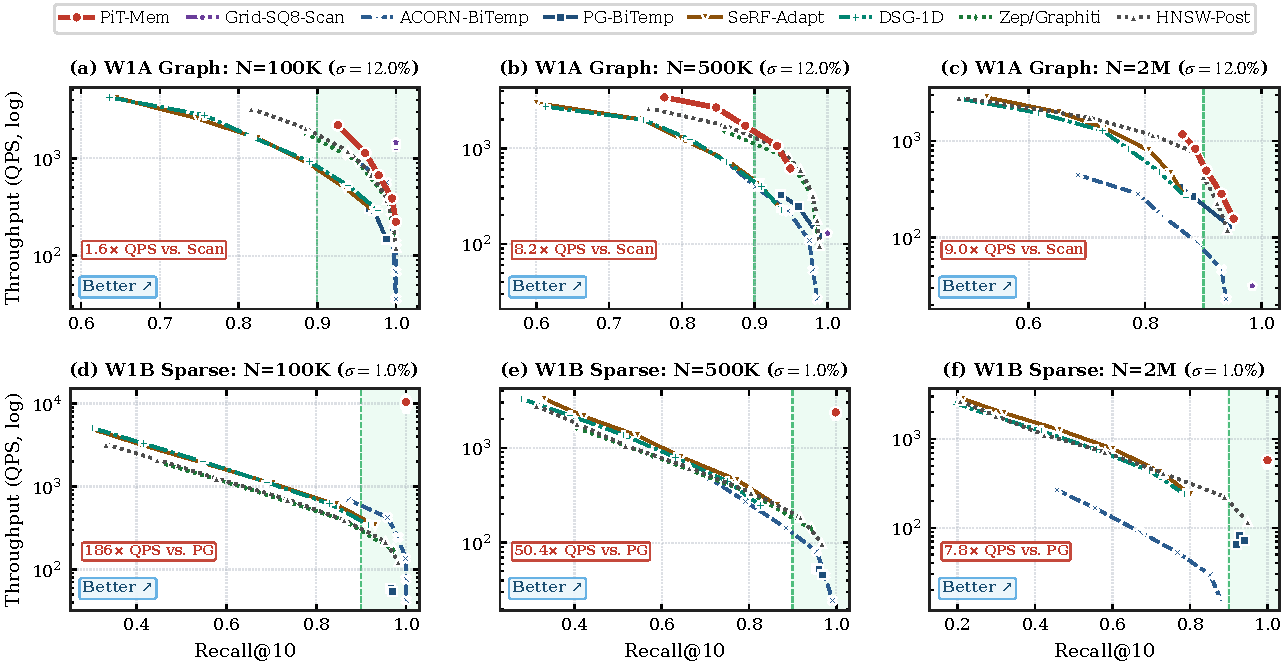
\includegraphics[width=0.92\textwidth]{figures/fig3_exp1_scalability.pdf}
    \Description{Two-row by three-column log-scale QPS vs Recall@10 Pareto curves across corpus scales up to 2,000,000 vectors for Workload 1A (moderate 12 percent selectivity) on top and Workload 1B (sparse 1 percent selectivity) on bottom.}
    \caption{Exp 1: Single-thread wall-clock QPS (log scale) vs.\ Recall@10 across $N \in \{100\text{K}, 500\text{K}, \MaxCorpusScale\}$ under Workload 1A ($\sigma \approx \ModSelectivityPct$, top row) and Workload 1B ($\sigma \approx 1.0\%$, bottom row). C++17 graph baselines (\texttt{ACORN-Style}, \texttt{HNSW-Flat}, \texttt{SeRF-Style}, \texttt{DSG-Style}, \texttt{Graphiti-Style}) are in-house bi-temporal adaptations.}
    \label{fig:exp1}
\end{figure*}

\TableExpOne

We evaluate PiT-Mem across six systems experiments:
\textbf{Q1 (\S\ref{sec:exp1})} multi-scale throughput across moderate ($\sigma \approx \ModSelectivityPct$) and sparse ($\sigma \approx 1.0\%$) regimes up to $N = \MaxCorpusScale$;
\textbf{Q2 (\S\ref{sec:exp2})} selectivity robustness across $\sigma \in [0.05\%, 50\%]$;
\textbf{Q3 (\S\ref{sec:exp3})} restatement throughput, calibrated Write+Read token modeling, and 3-hop bursts;
\textbf{Q4 (\S\ref{sec:exp4})} dual-protocol audit with \texttt{Qwen2.5-7B-Instruct}~\cite{yang2024qwen25};
\textbf{Q5 (\S\ref{sec:exp5})} RAP-Compact slot preservation, latency, and unified tiered search; and
\textbf{Q6 (\S\ref{sec:exp6})} streaming skew, NVMe checkpointing/WAL, \texttt{mmap} FP32 offload, and 12-thread mixed concurrency.

\subsection{Experimental Setup, FinPiT-Bench \& Baseline Scope}
\label{sec:setup}

\paragraph{Hardware, Provenance \& Measurement Protocol.}
All archived experiments ran on a Google Colab Pro instance equipped with an \ColabGPUName{} GPU (\ColabVRAMGB~GB VRAM), \ColabCPUCores{} Intel Xeon vCPUs (AVX2, FMA, OpenMP), \ColabRAMTotal{} RAM, and local NVMe SSD (\texttt{/content/local\_ssd}). All C++17 engines are compiled with \texttt{g++ -O3 -std=c++17 -mavx2 -mfma -fopenmp}. Primary throughput is single-thread sequential wall-clock QPS ($\text{1T QPS} = N_q / T_{\text{wall}}$), complemented by 12-thread QPS. Experiments ran modularly over identical corpus and query seeds (with \texttt{Exp 1} baseline rows reused across \texttt{BiT-HNSW} tuning iterations on the same corpus/query configuration).

\paragraph{FinPiT-Bench Seed Corpus \& Scaled Stream (\UniqueSeedPassages{} Unique Seeds).}
We assemble \textbf{FinPiT-Bench} from three public financial sources:
(1) \textbf{St.\ Louis Fed ALFRED}~\cite{anderson2006alfred}: $3{,}464$ multi-vintage observations across $7$ US macro series ($2019$--$2026$, $2{,}659$ revisions);
(2) \textbf{SEC EDGAR XBRL \& Form 8-K Item 4.02}: $33{,}224$ XBRL fact-version disclosures across $111$ issuers containing $3{,}086$ same-period XBRL revisions ($\ge 0.2\%$ change, $1{,}214$ post-\texttt{2025-01-01}) plus $75$ verified 2025--2026 Form 8-K Item 4.02 notices; and
(3) \textbf{Financial Disclosures \& News}: \HFUniquePassages{} deduplicated passages from \texttt{Financial-\allowbreak QA-10K}~\cite{singh2024finqa10k}, \texttt{Financial PhraseBank}~\cite{malo2014financial}, \texttt{Financial-\allowbreak News}~\cite{ashraq2022finnews}, \texttt{Finance-\allowbreak Alpaca}~\cite{bharti2023finalpaca}, and \texttt{Twitter-\allowbreak Fin-News}~\cite{zeroshot2022twitterfin}.
Scaling these \UniqueSeedPassages{} seeds to $N = \MaxCorpusScale$ bi-temporal versions ($\CorpusExpansionFactor$ reuse, encoded via \texttt{BAAI/\allowbreak bge-base-\allowbreak en-v1.5}~\cite{xiao2024cpack} into $768$-d unit vectors) combines seed passages with generated issuer/metric attributes and bi-temporal lifetimes ($53\%$ open-ended, $11\%$ evolved, $4\%$ restated). Over an $8{,}000$-vector sample, median $1$-NN cosine similarity is $\CorpusNNOneCosPfk$ with $\CorpusNearCloneRate$ pairs exceeding $\cos > 0.995$; intra-lineage SEC XBRL revisions exhibit median cosine $\IntraLineageSECCosPfk$ (P90 $\IntraLineageSECCosPninety$). For Exp 4, \textbf{Protocol~A} constructs $180$ post-cutoff 2025--2026 SEC XBRL revision trajectories and \textbf{Protocol~B} constructs $200$ anonymized \texttt{Firm\_Alpha} covenant templates (evaluating the first $120$ cases per protocol).

\paragraph{Evaluated Baselines \& Adaptation Scope.}
To ensure strict attribution, we distinguish external DBMSs from in-house C++17 bi-temporal adaptations:
(1) \textbf{\texttt{Grid-SQ8-Scan}}, a C++17 2D-grid AVX2 SQ8 scan baseline using geometrically growing, linearly extrapolated segments (not a strict graph-only ablation over BiT-HNSW's 416K Vitter segments);
(2) \textbf{\texttt{ACORN-Style}}, \textbf{\texttt{HNSW-Flat}}, \textbf{\texttt{SeRF-Style}}, and \textbf{\texttt{DSG-Style}}, in-house C++17 AVX2 bi-temporal adaptations implementing flat 2-hop predicate expansion (inspired by~\cite{patel2024acorn}), single-layer post-filtered proximity navigation (without HNSW's upper hierarchy~\cite{malkov2020hnsw}), and single-axis 1D prefix segment graphs over $t_v^s$ and $t_k^s$ sharing one C++ template (inspired by~\cite{zuo2024serf, peng2025dsg})---rather than unmodified upstream releases (our public repository additionally includes vendored upstream \texttt{nmslib/\allowbreak hnswlib} v0.8.0 bindings verified in unit tests);
(3) \textbf{\texttt{PG-BiTemp}}~\cite{pgvector2024, rajah2026postgraphrag}, PostgreSQL~16 + \texttt{pgvector} v0.8.0 (\texttt{halfvec(768)} HNSW \texttt{m=16} + composite B-Tree \texttt{(tk\_s, tv\_s) INCLUDE (tk\_e, tv\_e)}) with \texttt{shared\_\allowbreak buffers = 12GB}, \texttt{work\_\allowbreak mem = 256MB}, \texttt{VACUUM (ANALYZE)}, and \texttt{CHECKPOINT} up to $N = \PGMaxScale$; note that \texttt{PG-BiTemp} QPS reflects end-to-end Python client-server wall time over 50-query batches (including text-vector formatting, session GUCs, and 6 warmups per batch), whereas P99 reflects per-query post-warmup execution; and
(4) \textbf{Surrogate Policies} in Exp 4: \texttt{Latest-\allowbreak Summary (Graphiti-\allowbreak style)} (in-house HNSW+SQLite edge store appending an unbranched per-entity summary), \texttt{Overwrite (Mem0-\allowbreak style)}, and \texttt{Append-\allowbreak Only (GraphRAG-\allowbreak style)}, representing architectural policies rather than upstream deployments~\cite{rasmussen2025zep, chhikara2025mem0, edge2024graphrag}.

\subsection{Exp 1: Multi-Scale Throughput across Graph and Scan Regimes}
\label{sec:exp1}

Figure~\ref{fig:exp1} and Table~\ref{tab:exp1_detail} benchmark Workload~1A and Workload~1B up to $N = \MaxCorpusScale$ using perturbed queries sampled around calibrated temporal windows against C++ exact ground truth:

\paragraph{Workload 1A (Moderate Snapshot, $\sigma \approx \ModSelectivityPct$ --- Causal Graph Regime).}
At $N = \MaxCorpusScale$, BiT-HNSW triggers the \textbf{Dual-Budget Causal Graph on $\ModGraphTriggerPct$ of queries}, achieving \textbf{$\ModPiTMaxRecall$ Recall@10} at \textbf{$\ModPiTMaxQPS$~1T QPS} ($\ModPiTMaxMeanMs$~ms mean, $\ModPiTMaxPnnMs$~ms P99; $\ModSpeedupVsGridQPS$ the QPS and $\ModSpeedupVsGridPnn$ lower P99 than \texttt{Grid-SQ8-Scan} at $\ModGridScanQPS$~QPS / $\ModGridScanPnnMs$~ms), $\ModPiTFastRecall$ at $\ModPiTFastQPS$~1T / $\ModPiTMaxQPSConc$~12T QPS, and $\ModPiTPeakRecall$ peak Recall@10 at $\ModPiTPeakQPS$~1T QPS\@. Compared to our C++17 \texttt{ACORN-Style} adaptation ($\ModACORNQPS$~QPS, $\ModACORNRecall$ recall), PiT-Mem delivers $\ModSpeedupVsACORNQPS$ higher QPS, and outperforms \texttt{PG-BiTemp} ($\ModPGMaxQPS$~QPS, $\ModPGMaxPnnMs$~ms P99) by \textbf{$\ModSpeedupVsPGMaxQPS$ QPS} (\textbf{$\ModSpeedupVsPGMaxPnn$ lower P99}) at $2\text{M}$ scale.

\paragraph{Workload 1B (Sparse Historical Audit, $\sigma \approx 1.0\%$ --- Analytical Router).}
Across $N = 100\text{K}, 500\text{K}, \MaxCorpusScale$, Eq.~\eqref{eq:router} routes narrow $1\%$ queries to cell-pruned AVX2 SQ8 scanning ($\SparseRouterGraphPct$ graph share), delivering \textbf{$\PiTMaxRecall$ observed Recall@10} on this sampled sparse workload at \textbf{$\PiTMaxQPS$~1T QPS} ($\PiTMaxQPSConc$~12T QPS, $\PiTMaxMeanMs$~ms mean, $\PiTMaxPnnMs$~ms P99), matching \texttt{Grid-SQ8-Scan} ($\GridScanSparseMaxQPS$~QPS, $\GridScanSparseMaxPnnMs$~ms P99) without routing inversion. Note that because SQ8 re-ranks a finite top-$R$ pool, observed $100\%$ recall on this sample does not guarantee universal exactness. At $N = \MaxCorpusScale$, PiT-Mem achieves \textbf{$\SpeedupPGMaxQPS$ higher QPS} and \textbf{$\SpeedupPGMaxPnn$ lower P99} than \texttt{PG-BiTemp} ($\PGMaxScaleQPS$~QPS, $\PGMaxScalePnnMs$~ms P99, $4.87$~GiB on-disk relation+index size; build $\PiTBuildSec$~s vs.\ $\PGMaxBuildSec$~s), while our in-house flat \texttt{HNSW-Flat} ($\HNSWMaxRecall$ recall) and \texttt{ACORN-Style} ($\ACORNSparseRecall$ recall) degrade under narrow filtering.

\begin{figure}[t]
    \centering
    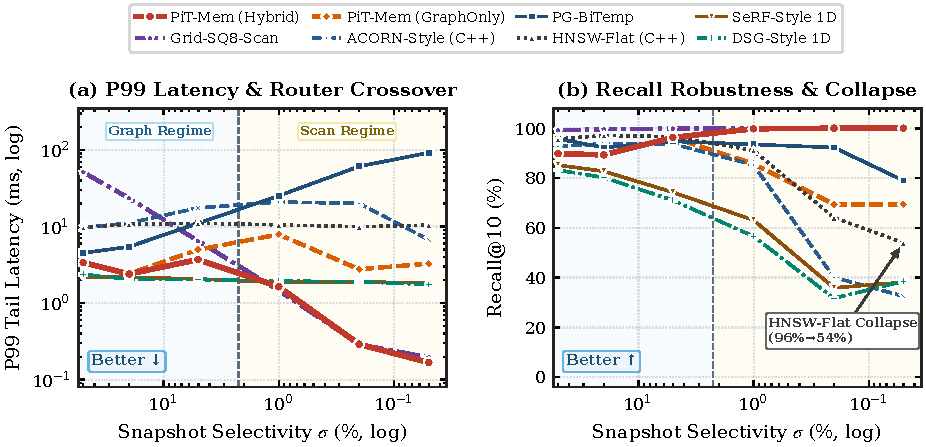
\includegraphics[width=\linewidth]{figures/fig4_exp2_selectivity.pdf}
    \Description{Two-panel selectivity sweep chart across interior temporal selectivities from 50 percent down to 0.05 percent showing P99 latency on left and Recall@10 on right.}
    \caption{Exp 2: P99 latency and Recall@10 across selectivities $\sigma \in [0.05\%, 50\%]$ ($N = \ExpTwoScale$), comparing \texttt{PiT-Mem} against \texttt{GraphOnly}, \texttt{Grid-SQ8-Scan}, \texttt{PG-BiTemp}, and C++17 graph adaptations.}
    \label{fig:exp2}
\end{figure}

\subsection{Exp 2: Selectivity Sweep \& Router Crossover}
\label{sec:exp2}

Figure~\ref{fig:exp2} sweeps selectivities $\sigma \in [0.05\%, 50\%]$ at $N = \ExpTwoScale$. On broad snapshots ($\sigma \in [5\%, 50\%]$), \texttt{PiT-Mem} tracks \texttt{GraphOnly} ($\BroadPitPnnMs$~ms P99, $\BroadPitQPS$~QPS, $\BroadPitRecall$ Recall@10 at $\sigma = 50\%$), beating \texttt{Grid-SQ8-Scan} ($\BroadScanPnnMs$~ms P99, $\BroadScanQPS$~QPS) by $\BroadScanSpeedup$ P99. Below the crossover ($\sigma \le 1\%$), \texttt{PiT-Mem} switches smoothly to cell-pruned AVX2 scanning, sustaining $\NarrowPitPnnMs$~ms P99 ($\NarrowPitQPS$~QPS, $\NarrowPitRecall$ observed recall) at $\sigma \approx 0.05\%$, whereas \texttt{HNSW-Flat} ($\NarrowHNSWRecall$ recall) and \texttt{ACORN-Style} ($\NarrowACORNRecall$ recall) suffer percolation collapse.

\begin{figure*}[t]
    \centering
    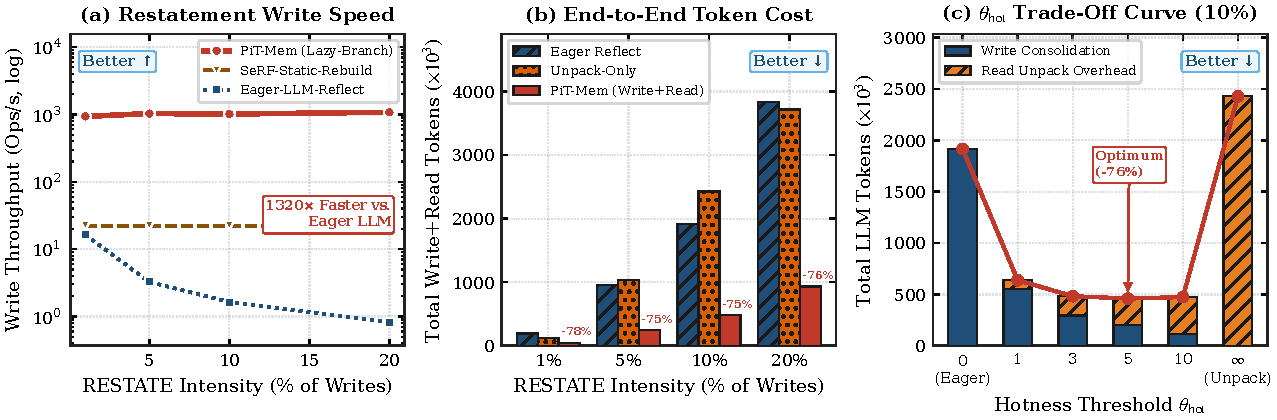
\includegraphics[width=0.92\textwidth]{figures/fig5_exp3_restate.pdf}
    \Description{Three-panel restatement maintenance plot showing measured C++ write attempts vs calibrated eager/rebuild models on left, calibrated write+read LLM token accounting model in center, and hotness threshold U-curve on right.}
    \caption{Exp 3: (a) Attempted C++ write rate ($1\%$--$20\%$ \texttt{RESTATE}) vs.\ calibrated \texttt{Static Rebuild} and \texttt{Eager-LLM} models; (b) calibrated Write+Read LLM token accounting model; (c) modeled $\theta_{\text{hot}} \in \{0, 1, 3, 5, 10, \infty\}$ trade-off curve.}
    \label{fig:exp3}
\end{figure*}

\subsection{Exp 3: Restatement Cost Model \& 3-Hop Clustered Bursts}
\label{sec:exp3}

Figure~\ref{fig:exp3} evaluates provenance maintenance under $1\%$--$20\%$ \texttt{RESTATE} churn followed by $\text{Zipf}(1.38)$ post-restatement reads. We separate directly timed C++ metadata operations from our \textbf{calibrated LLM cost model}: on the C++ write loop (Figure~\ref{fig:exp3}a), \texttt{PiT-Mem} sustains $\RestateWriteOps$ attempted mixed-stream ops/s ($\RestateWritePfkUs~\mu$s P50, $\RestateWritePnnUs~\mu$s P99) via $O(1)$ SoA death updates and reverse-BFS tainting, whereas \texttt{Static Rebuild} (extrapolated from 50K rebuilds amortized over 250-op batches) estimates $\RestateStaticOps$~ops/s and \texttt{Eager-LLM} (modeled from measured \texttt{Qwen2.5-7B-Instruct} per-call consolidation latency) estimates $\RestateEagerOps$~ops/s at $10\%$ churn. Because write loops in this archived run counted attempted operations before explicit \texttt{committed} return flags were added to \texttt{apply\_evolve} (verified zero-rejection in our updated unit tests), we report this rate as attempted ops/s. Under our calibrated token accounting model (Figure~\ref{fig:exp3}b--c, charging calibrated per-reflection consolidation tokens and per-hit unpack prompt overhead), \texttt{Eager-LLM} ($\theta_{\text{hot}}=0$) incurs $\EagerWriteTokensTenPct$ modeled write tokens at $10\%$ churn and \texttt{Unpack-Only} ($\theta_{\text{hot}}=\infty$) incurs $\UnpackReadExtraTokensTenPct$ modeled extra read tokens; \texttt{PiT-Mem} reaches its modeled minimum at $\theta_{\text{hot}}=5$ ($459{,}846$ tokens, $-76.0\%$) and averages $\AvgTokenSavings$ estimated savings at default $\theta_{\text{hot}}=3$.

\paragraph{Exp 3B: Directly Measured 3-Hop Clustered Restatement Bursts.}
To test Algorithm~\ref{alg:mvcc}'s adaptive refill mechanism directly in C++, we construct an adversarial 3-hop provenance hierarchy (\textsc{Raw} $\to$ L1 $\to$ L2 $\to$ L3 \textsc{Reflect}) where bursts of $8, 16, 24,$ and $32$ top-ranked reflections are simultaneously tainted and unpack into distant leaves. Static over-fetching ($k_{\text{fetch}} = 22$ for $k=10$) starves clean candidates beyond burst size $12$, dropping clean Recall@10 to \textbf{$\BurstTwentyFourStaticRecall$} (burst $24$) and \textbf{$\BurstThirtyTwoStaticRecall$} (burst $32$). Algorithm~\ref{alg:mvcc}'s adaptive $k_{\text{fetch}}$ doubling preserves \textbf{$\BurstTwentyFourAdaptRecall$} and \textbf{$\BurstThirtyTwoAdaptRecall$ clean Recall@10} in $\BurstThirtyTwoAdaptRounds$ mean refill rounds ($\BurstThirtyTwoAdaptPnnMs$~ms P99, $0.0\%$ STR, $|\mathcal{O}| \le k$).

\begin{figure}[t]
    \centering
    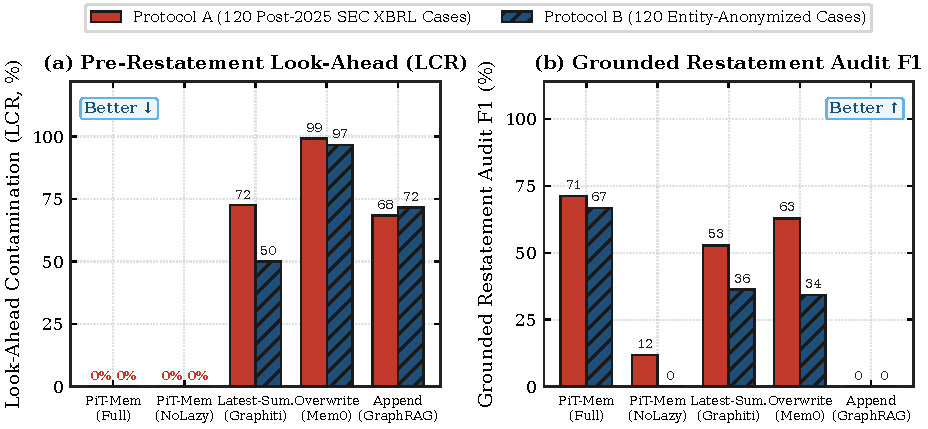
\includegraphics[width=\linewidth]{figures/fig6_exp4_leakage.pdf}
    \Description{Two-panel grouped bar chart comparing Pre-Restatement Look-Ahead Contamination Rate on left and Grounded Restatement Audit F1 on right across Protocol A and Protocol B for surrogate memory policies.}
    \caption{Exp 4: Look-Ahead Contamination Rate (LCR, left) and Grounded Restatement Audit F1 (right) across the first 120 cases per protocol using \texttt{Qwen2.5-7B-Instruct} over surrogate memory policies.}
    \label{fig:exp4}
\end{figure}

\TableExpFour

\subsection{Exp 4: Look-Ahead Leakage \& Restatement Audit F1}
\label{sec:exp4}

Figure~\ref{fig:exp4} and Table~\ref{tab:exp4} evaluate $240$ balanced pre-/post-restatement queries per protocol ($120$ cases each from Protocols~A and B; $480$ queries/policy) with \texttt{Qwen2.5-7B-Instruct}~\cite{yang2024qwen25}, comparing PiT-Mem against three in-house surrogate memory policies (rather than unmodified upstream frameworks). The \texttt{Overwrite} (\texttt{Mem0-style}) policy exhibits $\MemZeroLCR$ LCR on Protocol~A; \texttt{Append-Only} (GraphRAG-style) leaks future revisions ($\NaiveRAGLCRA$ LCR) and leaves invalidated records active ($100.0\%$ stale taint); and \texttt{Latest-Summary} (Graphiti-style) leaks post-restatement state via unbranched summaries ($\GraphitiLCR$ / $\GraphitiLCRB$ LCR). Omitting Lazy-Branch (\texttt{PiT-Mem w/o Lazy-Branch}) keeps $\text{LCR} = 0\%$ but leaves $\NoLazyStaleA$--$\NoLazyStaleB$ of post-restatement reads tainted, collapsing Audit F1 to $\NoLazyFOneA$ / $\NoLazyFOneB$. \textbf{PiT-Mem (Full)} achieves \textbf{$\PiTLCR$ LCR}, \textbf{$0.0\%$ Stale Taint}, and \textbf{$\PiTAuditFOneA$} / \textbf{$\PiTAuditFOneB$ Audit F1}. Three of the $120$ Protocol~A originals already mention prior restatements under the binary prompt, imposing a conservative ceiling on Audit F1; we also omit synthetic return-shock Sharpe ratios from headline claims (retaining an illustrative simulation only in the archived CSV).

\begin{figure}[t]
    \centering
    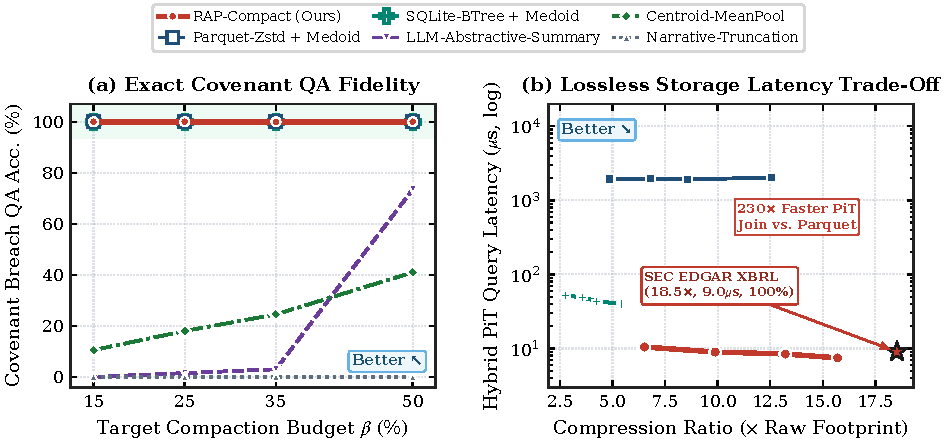
\includegraphics[width=\linewidth]{figures/fig7_exp5_compact.pdf}
    \Description{Two-panel chart showing template anchor-check accuracy across compaction budgets on left, and query latency vs compression ratio across RAP-Compact, SQLite-BTree, and Parquet-Zstd on right.}
    \caption{Exp 5: (a) Entity-scoped template anchor preservation across $\beta \in [15\%, 50\%]$; (b) query latency ($\mu$s) vs.\ compression ratio across resident C++ \texttt{RAP-Compact} (SQ8), in-memory \texttt{SQLite-BTree} (FP32), and per-request \texttt{Parquet-Zstd} file scans (FP32).}
    \label{fig:exp5}
\end{figure}

\TableExpFive

\subsection{Exp 5: RAP-Compact Slot Preservation \& Tiered Retrieval}
\label{sec:exp5}

Figure~\ref{fig:exp5} and Table~\ref{tab:exp5} evaluate structured slot preservation and lookup latency on the $200$ generated Protocol~B covenant templates and XBRL-derived templated disclosures. All three extractor-backed stores (\texttt{RAP-Compact}, \texttt{SQLite-BTree + Medoid}~\cite{hipp2020sqlite}, and \texttt{Parquet-Zstd + Medoid}~\cite{apacheparquet2024}) preserve $100.0\%$ of extracted covenant slots across $\beta \in [15\%, 50\%]$ on entity-scoped template checks (where known financial actuals are supplied alongside extracted covenant thresholds; XBRL-derived disclosures are verified within display-rounding tolerance). By contrast, lossy text/centroid baselines lose non-medoid thresholds, though note that the archived \texttt{LLM-Abstractive-Summary} run truncated group inputs at $2{,}400$ characters with per-document output caps, so its $\LLMSumCovenantQA$ score reflects that constrained prompt budget rather than an upper bound on LLM summarization.

On query latency at $\beta = 25\%$ ($\RAPCompRatio$ compression; $\RAPMaxCompRatio$ at $\beta = 15\%$), resident C++ \texttt{RAP-Compact} executes entity-scoped SQ8 + 56B anchor lookup in \textbf{$\RAPQueryLatUs~\mu$s}---\textbf{$\RAPSpeedupVsSQLite$ faster than in-memory \texttt{SQLite-BTree}} ($\SQLiteQueryLatUs~\mu$s, $4.3\times$ compression, over FP32 medoids) and $9.0~\mu$s ($\WildSECCompRatio$ compression) on XBRL-derived disclosures. While per-request \texttt{Parquet-Zstd} file filtering incurs $\ParquetQueryLatUs~\mu$s due to repeated PyArrow file opening, row-group decoding, and FP32 medoid scoring, we treat in-memory \texttt{SQLite-BTree} as the primary resident comparison point given the differing execution models.

\paragraph{Exp 5C: Unified Tiered Search (\textup{\texttt{query\_tiered\_pit}}).}
Evaluating $200$ queries spanning compacted historical indentures (\textsc{Compact}) alongside live hot-tier \texttt{BiT-HNSW} restatements and amendments, \texttt{Hot-Only} covers $\TieredHotOnlyQA$ of target entity slots and \texttt{Cold-Only} covers $\TieredColdOnlyQA$, whereas unified \texttt{query\_tiered\_pit} merges hot/cold candidates on $[0, 4]$ with \texttt{source\_mem\_id} deduplication to achieve \textbf{$\TieredUnifiedQA$ cross-tier entity-slot coverage} ($\TieredUnifiedSTR$ hot-origin STR) in $\TieredUnifiedMeanUs~\mu$s mean ($\TieredUnifiedPnnUs~\mu$s P99).

\TableExpSix
\TableExpSixSys

\subsection{Exp 6: Streaming Skew, Durability, Cold-FP32 Offload \& Concurrency}
\label{sec:exp6}

Tables~\ref{tab:exp6} and~\ref{tab:exp6_sys} evaluate four systems dimensions:
(1) \textbf{Streaming Skew Ablation (Exp~6A, Table~\ref{tab:exp6})}: On chronological streams ($N = \StreamScale$) without future timestamp knowledge, a frozen $5\%$-bootstrap grid (\texttt{Static-Frozen-BootGrid}) piles $\FrozenCellPileupPct$ of arrivals into cell $(15, 15)$ ($\FrozenQPS$~QPS, $\FrozenPnnMs$~ms P99). Bounded $416\text{K}$ causal macro-segments ($\StreamSegments$ segments) with Vitter lag-convolution calibration and the $>20\%$ skew guard eliminate $(15, 15)$ pile-up ($0.0\%$), cap sealed/active-tail max cell share at $\StreamSealedMaxCellPct$/$\StreamMaxCellPct$, and achieve $\StreamQPS$~QPS ($\StreamPnnMs$~ms P99, $\StreamSpeedupVsFrozen$ over frozen bootstrap, matching hindsight \texttt{Offline-Oracle-Grid} at $\OracleQPS$~QPS).
(2) \textbf{NVMe Checkpointing \& CRC-32 WAL (Exp~6B)}: At $N = \MaxCorpusScale$, PiT-Mem writes its $\NVMeSnapGiB$~GiB CSR/SoA snapshot in \textbf{$\NVMeSaveSec$~s} ($\NVMeSaveMiBs$~MiB/s), restores it into heap buffers via sequential \texttt{mmap} in \textbf{$\NVMeLoadWarmSec$~s} ($\NVMeLoadWarmGiBs$~GiB/s), and replays a $1{,}000$-frame CRC-32 WAL in \textbf{$\NVMeWALReplayMs$~ms} (verified for record-count parity $N + 200$ at $2\text{M}$ scale; torn-tail transaction rollback and full state/timestamp/vector parity are verified in supplementary unit tests).
(3) \textbf{POSIX \texttt{mmap} Cold-FP32 Offload (Exp~6C, Table~\ref{tab:exp6_sys} top)}: Offloading $3{,}072$~B/rec FP32 vectors at $\OffloadWriteMBs$~MB/s reduces counted core index arrays from $\PiTMemGiB$~GiB to $\CoreIndexRAMGiB$~GiB ($\CoreIndexBytesPerRec$~B/rec, excluding auxiliary hash-map metadata and OS page-cache residency). Warm-cache throughput matches All-RAM ($\OffloadWarmModQPS$ vs.\ $\OffloadAllRamModQPS$ on W1A; $\OffloadWarmSparseQPS$ vs.\ $\OffloadAllRamSparseQPS$ on W1B). After issuing per-microbatch advisory eviction requests (\texttt{POSIX\_FADV\_DONTNEED} + \texttt{MADV\_DONTNEED}), PiT-Mem sustains $\OffloadColdModQPS$~1T / $\OffloadColdModQPSConc$~12T QPS ($\OffloadColdModPnnMs$~ms P99) on W1A and $\OffloadColdSparseQPS$~1T / $\OffloadColdSparseQPSConc$~12T QPS ($\OffloadColdSparsePnnMs$~ms P99) on W1B; because OS residency and major-fault counters were not instrumented in this archived run, these rows represent post-advisory-eviction performance rather than verified cold-device I/O.
(4) \textbf{Phase-Fair Concurrent Mixed Stress (Exp~6D, Table~\ref{tab:exp6_sys} bottom)}: Under $12$ reader threads running concurrently with a mixed-stream writer triggering live \texttt{MacroSegment} rollovers ($\ConcPerRunRollovers$ per run, $\ConcTotalRollovers$ total; $N = \ConcScale$), \texttt{PhaseFairSharedMutex} sustains \textbf{$\ConcTwelveMixedQPS$~mixed reader QPS} ($\ConcTwelveMixedPnnMs$~ms P99; vs.\ $\ConcTwelveROQPS$~QPS read-only) alongside $\ConcTwelveWriterOps$ attempted writer ops/s with \textbf{$\ConcTotalViolations$ isolation or cardinality violations}.

\paragraph{Threats to Validity \& Scope.}
We note four boundaries of our archived evaluation: (i) Exp~1--2 graph baselines are in-house C++17 bi-temporal adaptations rather than unmodified upstream releases, and Exp~4 evaluates surrogate policies on $120$ cases/protocol; (ii) Exp~3 token savings and \texttt{Eager-LLM} write rates use a calibrated model rather than $10{,}000$ live synchronous LLM re-consolidations; (iii) Exp~5 evaluates template-bound slot preservation with known actuals rather than unconstrained contract QA, comparing distinct storage/vector paths across \texttt{RAP-Compact}, \texttt{SQLite-BTree}, and \texttt{Parquet-Zstd}; and (iv) counted array memory ($1{,}032$~B/rec) excludes auxiliary hash maps and OS page cache, while Exp~6C advisory evictions do not instrument physical NVMe major faults. Our public repo includes post-audit C++17 fixes (explicit \texttt{committed} counters, disjoint slice IDs via \texttt{HIST\_SLICE\_BASE}, bit-exact torn-WAL checks, and vendored \texttt{hnswlib} v0.8.0 bindings) verified in unit tests.

\section{Related Work}
\label{sec:related}

\paragraph{Temporal \& Bi-Temporal Access Methods.}
SQL:2011 temporal semantics~\cite{snodgrass1999developing, kulkarni2012sql2011, jensen1999temporal, salzberg1999comparison} motivated TSB-Tree~\cite{lomet1989tsbtree}, MVBT~\cite{becker1996mvbt}, bitemporal R-trees~\cite{kumar1998bitemporal}, temporal alignment~\cite{dignos2012temporal}, SAP HANA's Timeline Index~\cite{kaufmann2013timeline}, and HINT~\cite{christodoulou2022hint}. Scalar temporal indexes cannot prune high-dimensional vector spaces without linear scans or decoupled post-filtering.

\paragraph{MVCC \& Agent Memory.}
Classic MVCC engines (Hekaton~\cite{larson2011hekaton}, HyPer~\cite{neumann2015hyper}, MVCC studies~\cite{wu2017mvcc}, LeanStore~\cite{leis2018leanstore}) pair version chains or swizzling with phase-fair locks~\cite{brandenburg2010phasefair}; provenance semirings~\cite{green2007provenance} formalize lineage; and AeonG~\cite{hou2024aeong} tracks 1D transaction-time deltas. Agentic memory systems (Generative Agents~\cite{park2023generative}, MemGPT~\cite{packer2023memgpt}, MemoryBank~\cite{zhong2024memorybank}, Mem0~\cite{chhikara2025mem0}, and GraphRAG~\cite{edge2024graphrag, li2026agenticmemory, wu2025longmemeval}) lack bi-temporal isolation. Look-Ahead-Bench~\cite{benhenda2026lookahead} audits parametric bias, while Zep/\allowbreak Graphiti~\cite{rasmussen2025zep} and \texttt{post-graph-rag}~\cite{rajah2026postgraphrag} layer four timestamps atop graphs or \texttt{pgvector}~\cite{pgvector2024} without causal-prefix ANNS or lazy-branch repair.

\paragraph{Filtered, Range-Filtered \& Disk-Tiered ANNS\@.}
High-dimensional ANNS spans graph navigation (HNSW~\cite{malkov2020hnsw}), quantization (PQ~\cite{jegou2011pq}, RaBitQ~\cite{gao2024rabitq}), vector DBMSs (Milvus~\cite{wang2021milvus}), and SSD-tiered indexes (DiskANN~\cite{subramanya2019diskann}, FreshDiskANN~\cite{singh2021freshdiskann}, SPANN~\cite{chen2021spann}, Starling~\cite{wang2024starling}). Predicate-filtered graphs (Filtered-DiskANN~\cite{gollapudi2023filtereddiskann}, ACORN~\cite{patel2024acorn}) handle static labels or moderate predicates, whereas SeRF~\cite{zuo2024serf}, UNIFY~\cite{liang2024unify}, and DSG~\cite{peng2025dsg} index one immutable scalar key. BiT-HNSW co-designs Vitter-calibrated~\cite{vitter1985reservoir} streaming 2D birth macro-segments, $O(1)$ SoA AVX2 mutable right-endpoint filtering, dual-budget causal graphs, analytical routing, and POSIX \texttt{mmap} cold-FP32 tiering.

\section{Conclusion}
\label{sec:conclusion}

We presented \textbf{PiT-Mem}, a persistent bi-temporal storage and indexing engine for look-ahead-free agentic memory. Uniting streaming \textbf{Causal Macro-Segment BiT-HNSW} ($\CoreIndexBytesPerRec$~B/rec counted core arrays, POSIX \texttt{mmap} FP32 offload, analytical routing, CRC-32 WAL), phase-fair adaptive \textbf{Lazy-Branch MVCC}, and \textbf{RAP-Compact}, PiT-Mem achieves $\ModPiTMaxRecall$ Recall@10 at $\ModSpeedupVsGridQPS$ QPS over \texttt{Grid-SQ8-Scan} ($\ModSpeedupVsPGMaxQPS$ over \texttt{PG-BiTemp} at $\MaxCorpusScale$ on W1A; $\SpeedupPGMaxQPS$ QPS / $\SpeedupPGMaxPnn$ P99 on W1B with $\PiTMaxRecall$ observed sparse recall), $\ConcTwelveMixedQPS$ 12T mixed reader QPS with zero isolation violations, $\PiTLCR$ LCR across $240$ dual-protocol audit cases ($\AvgTokenSavings$ modeled token savings), and $100.0\%$ slot preservation on template checks at $\RAPQueryLatUs~\mu$s ($\RAPSpeedupVsSQLite$ faster than in-memory \texttt{SQLite-BTree}).

\clearpage
\bibliographystyle{ACM-Reference-Format}
\bibliography{references}

\end{document}
\endinput
